\documentclass[12pt,letterpaper]{article}

% ── Geometry ──────────────────────────────────────────────────────────
\usepackage[margin=1in,headheight=14pt]{geometry}

% ── Fonts (XeLaTeX) ──────────────────────────────────────────────────
\usepackage{fontspec}
\setmainfont{DejaVu Serif}
\usepackage{xeCJK}
\setCJKmainfont{Noto Serif CJK SC}

% ── Spacing ──────────────────────────────────────────────────────────
\usepackage{setspace}
\onehalfspacing
\usepackage{parskip}

% ── Math ─────────────────────────────────────────────────────────────
\usepackage{amsmath}
\usepackage{amssymb}
\usepackage{unicode-math}

% ── Tables ───────────────────────────────────────────────────────────
\usepackage{booktabs}
\usepackage{longtable}
\usepackage{array}
\usepackage{multirow}
\usepackage{calc}

% ── Figures ──────────────────────────────────────────────────────────
\usepackage{graphicx}
\usepackage{float}
\usepackage[section]{placeins}

% ── Captions ─────────────────────────────────────────────────────────
\usepackage[font=small,labelfont=bf]{caption}

% ── Headers ──────────────────────────────────────────────────────────
\usepackage{fancyhdr}
\pagestyle{fancy}
\fancyhf{}
\fancyhead[L]{\small\itshape Pagadala}
\fancyhead[R]{\small\itshape Education of Nations}
\fancyfoot[C]{\thepage}
\renewcommand{\headrulewidth}{0.4pt}

% ── Colors and hyperlinks ─────────────────────────────────────────────
\usepackage{xcolor}
\usepackage[colorlinks=true,linkcolor=blue!60!black,citecolor=blue!60!black,urlcolor=blue!60!black,
  pdftitle={Education of Nations: Against the Wealth of Nations},
  pdfauthor={Krishna Pagadala}]{hyperref}

% ── Code / script references ─────────────────────────────────────────
\usepackage{listings}
\lstset{basicstyle=\small\ttfamily,breaklines=true}

% ── Tight list (pandoc requirement) ──────────────────────────────────
\providecommand{\tightlist}{%
  \setlength{\itemsep}{0pt}\setlength{\parskip}{0pt}}

% ── CSQuotes for proper quoting ──────────────────────────────────────
\usepackage{csquotes}

% ── Section formatting ───────────────────────────────────────────────
\usepackage{titlesec}
\titleformat{\section}{\Large\bfseries}{\thesection.}{0.5em}{}
\titleformat{\subsection}{\large\bfseries}{\thesubsection}{0.5em}{}
\titleformat{\subsubsection}{\normalsize\bfseries}{\thesubsubsection}{0.5em}{}

% ══════════════════════════════════════════════════════════════════════
% DOCUMENT
% ══════════════════════════════════════════════════════════════════════

\begin{document}

% ── Title ─────────────────────────────────────────────────────────────
\begin{titlepage}
\begin{center}
\vspace*{2cm}
{\LARGE\bfseries Education of Nations:\\Against the Wealth of Nations\par}
\vspace{1.5cm}
{\large Krishna Pagadala\par}
\vspace{0.5cm}
{\normalsize\itshape Working paper, 2026\par}
\vspace{1cm}
{\small\itshape In memory of Richard A.\ Easterlin (1926--2024), who asked the right question.\par}
\vspace{1cm}
\end{center}

\begin{abstract}
\noindent Development theory since Adam Smith has treated education as one input
among many --- sometimes crediting income growth, sometimes direct state
provision. Both are wrong about cause. Education is the cause of human
development: the only input without which no other mechanism operates,
and the only one that survives its own removal test. Remove income, and
education still works: Bangladesh reached longer lives and fewer
children per woman than the 1960 United States --- at \$1,159 per
capita. Remove provision, and education still works: South Korea and
Taiwan achieved development with minimal welfare states. Remove
education, and nothing works. By 2022, 154 countries representing 80\%
of the world's population have crossed both thresholds. The remaining
20\% is concentrated in sub-Saharan Africa, plus Pakistan, Afghanistan,
and Yemen as the largest exceptions outside Africa.

In 187-country panel data (WCDE v3, 1960--2015) with country fixed
effects and a 25-year generational lag, the decisive evidence is
threefold. First, education predicts future life expectancy while GDP
does not: education explains 47\% of within-country variation in life
expectancy one generation forward, GDP explains 17\% --- but when GDP is
residualized against education (removing education's contribution to
income), GDP's independent predictive power falls to near zero
($R^2 < 0.025$, $p > 0.1$) on every outcome tested: life
expectancy, fertility, child mortality, and the next generation's
education. Second, education's predictive power persists across three
generational depths while income's collapses within one generation
(Figure 3). Third, at no point in any country's trajectory does
educational attainment decline from one generation to the next. Parental
Transmission (PT) makes the gains irreversible; agency --- the household
decisions of educated adults --- produces the development outcomes
\textasciitilde25 years later.

Sen's distinction between growth-mediated and support-led security
(Drèze \& Sen, 1989) --- the most influential framework in development
policy --- classifies pathways by whether welfare arrives through income
or through state provision, implicitly treating both as independent
mechanisms. Neither is. Both are downstream of education. The two
categories are the same mechanism producing different surface appearances
depending on expansion speed and the presence of functioning markets.
Every canonical case crossed the development threshold at the interval
that prior education investment predicts, not from when provision
programmes were introduced. These findings extend Easterlin (1981) and
Lutz \& Kebede (2018) to within-country identification of the
generational mechanism.

\vspace{0.5em}
\noindent\textbf{Keywords:} education; generational transmission; human
development; Preston Curve; PT; agency; income-led development;
provision-led development; education policy
\end{abstract}

\thispagestyle{empty}
\end{titlepage}

\setcounter{page}{2}

\section{Introduction}\label{introduction}

The error has a specific origin. In 1776, Adam Smith observed the pin
factory and built a theory of wealth from the division of labour. He
never asked where the educated workforce came from that made division of
labour possible. Smith was born in Kirkcaldy in 1723, twenty-seven years
after Scotland's Education Act of 1696 codified John Knox's programme of
universal parish schooling into statute. The workforce he observed was
the product of 150 years of deliberate educational investment --- the
grandchildren of Knox's first generation of pupils. Smith took educated
labour as given. The tradition he founded inherited that assumption, and
development economics has been working backwards from it ever since.

Smith's error was not a personal failure of observation. It was
structurally invisible. For the entire pre-industrial period --- roughly
ten thousand years from agriculture to the steam engine --- the world
was Malthusian: total wealth was approximately fixed, and any gain by
one group came at the expense of another. In a zero-sum world, hierarchy
suppresses mass education rationally --- the literate peasant is a
danger, not an asset, when there is no new wealth to create. The
equilibrium was self-reinforcing: no surplus to fund mass schooling, no
mass schooling to generate surplus. What broke it was a contingent
alignment. John Knox, for purely religious reasons --- every person must
read the Bible --- broke the knowledge monopoly in 1560, two centuries
before the steam engine. Scotland's education did not make Scotland
rich; the zero-sum constraint held. But when fossil fuels arrived, they
encountered a population already educated enough to deploy the new
energy productively. Smith stood at exactly this inflection point ---
the first generation in human history where educated labour produced
visible, compounding wealth --- and mistook the output (division of
labour, productivity) for the cause. The countries that remained in
inertia after 1800 were not uniformly missing energy --- many possessed
coal and oil deposits. What they were missing was an educated workforce
to convert energy into development. Japan, with negligible domestic
fossil fuels, industrialised within a generation of the Meiji education
reforms; Nigeria, sitting on one of the world's largest oil reserves,
did not.

Easterlin (1981) was the first to ask the question Smith did not: ``Why
Isn't the Whole World Developed?'' His answer --- the binding constraint
was the absence of mass schooling systems, whose historical distribution
tracked the Protestant Reformation's literacy imperative --- pointed
directly at the omission. Lutz \& Kebede (2018) showed that the Preston
Curve, the canonical relationship between income and life expectancy, is
tighter when education replaces income on the x-axis: what looked like
``wealth buys health'' was education proxying through income all along.
Both identified the correction. Neither stated the conclusion it
implies.

This paper states it. Education is the cause of human development.
Income is downstream. Direct provision is downstream. In \emph{Hunger
and Public Action} (Drèze \& Sen, 1989), Sen codified the distinction
that became the most influential framework in development policy for
four decades: some countries secure welfare through economic growth
(growth-mediated security); others through direct state provision
regardless of income (support-led security). Kerala, Sri Lanka, and
China were the paradigm cases of the second type --- populations with
welfare outcomes far above what their incomes predicted. This taxonomy
is the most consequential expression of the assumption Smith introduced
--- that education can be taken as given.

My argument is not that Sen overlooked education, but that his taxonomy
--- by classifying pathways as either growth-mediated or support-led ---
implicitly treats both income and provision as independent mechanisms.
They are not. Both are downstream of education. Sen's two categories are
the same mechanism --- education --- producing two different surface
appearances depending on the speed of educational expansion and the
presence of functioning markets. Where educational expansion is fast and
markets function, the mechanism produces rapid visible income growth;
that income growth gets credited as the cause. Where expansion is slow
and markets are absent, income growth is invisible; state services are
the only observable welfare activity and they get credited instead. The
taxonomy describes how resources flow through different institutional
channels (markets vs.~state services), not the underlying cause of
development --- but development policy read it as causation, and
allocated accordingly. International aid now favours health over
education at 2--3× (OECD DAC, 2022), and the SDGs rank education fourth
--- behind hunger, which the UN's own Human Development Index does not
include.

Education is the cause --- the only input that cannot be removed by
economic collapse, state failure, or external shock. Income can be
removed by economic crisis; provision can be removed by fiscal collapse;
both happen routinely. Education cannot be removed because it is
embodied in people, not stored in budgets or institutions. The removal
tests (Section 4; Section 7) confirm this asymmetry across every
available natural experiment. No other input survives its own removal.


\section{Defining Development}\label{defining-development}

I operationalize development concretely: a country is developed when it
has simultaneously achieved a \textbf{total fertility rate (TFR) below
3.65} and \textbf{life expectancy \textgreater{} 69.8 years} --- the
1960 United States values (World Bank WDI).

This definition is deliberate and theoretically motivated on three
grounds.

First, 1960 is the natural baseline for the post-colonial world.
Seventeen African countries gained independence in 1960 alone; the
decade marks the inflection point at which most of the developing world
began its independent trajectory. The development question is precisely:
from the moment of decolonization, which countries achieved human
welfare outcomes that surpassed the global hegemon? That is a
theoretically precise question, not an arbitrary one.

Second, the USA in 1960 was the unambiguous global hegemon --- the
world's largest economy and dominant military power for fifteen years. A
country that crosses both thresholds --- lower TFR, higher life
expectancy --- has surpassed the richest, most powerful nation on earth
on the metrics that matter for human welfare. The bar is meaningful.

Third, the USA in 1960 was itself still mid-demographic transition. Its
TFR of 3.65 is the baby boom peak --- the country had not yet completed
the fertility transition (it crossed in 1972). Crossing below that
threshold means going further than the hegemon had gone, not meeting a
low standard.

The definition measures what matters. TFR and LE are chosen because they
have intrinsic value: how long people live and whether women control
their own fertility are ends in themselves, not proxy variables selected
to flatter a model. They require neither high income nor a particular
type of government to achieve, making them appropriate for cross-regime,
cross-income comparison. That education predicts them is an empirical
finding, not a design choice. The circularity objection --- that I chose
outcomes education predicts --- is addressed by Table A4: crossing dates
under three threshold specifications shift by 6--35 years but the
ordering and the PT-prediction alignment hold. The shift range is itself
diagnostic: countries with high expansion rates cross any threshold
within 6--7 years. GDP is excluded by design: measuring development
through income would beg the question against an education-primary
account.

The countries that had already crossed both thresholds by 1960 were
those with the longest prior histories of mass education: Scandinavia,
the Netherlands, France, Switzerland, the United Kingdom, Australia, and
New Zealand. Japan --- despite a TFR of 2.0 --- had life expectancy of
67.7, just below the threshold; it crossed in 1964. The development
dating analysis is robust to alternative threshold specifications
(Appendix Table A4).

By 2022, 154 countries have crossed both thresholds, representing 80\%
of the world's population. Figure 1 traces this accumulation over time.

\begin{figure}[htbp]
\centering
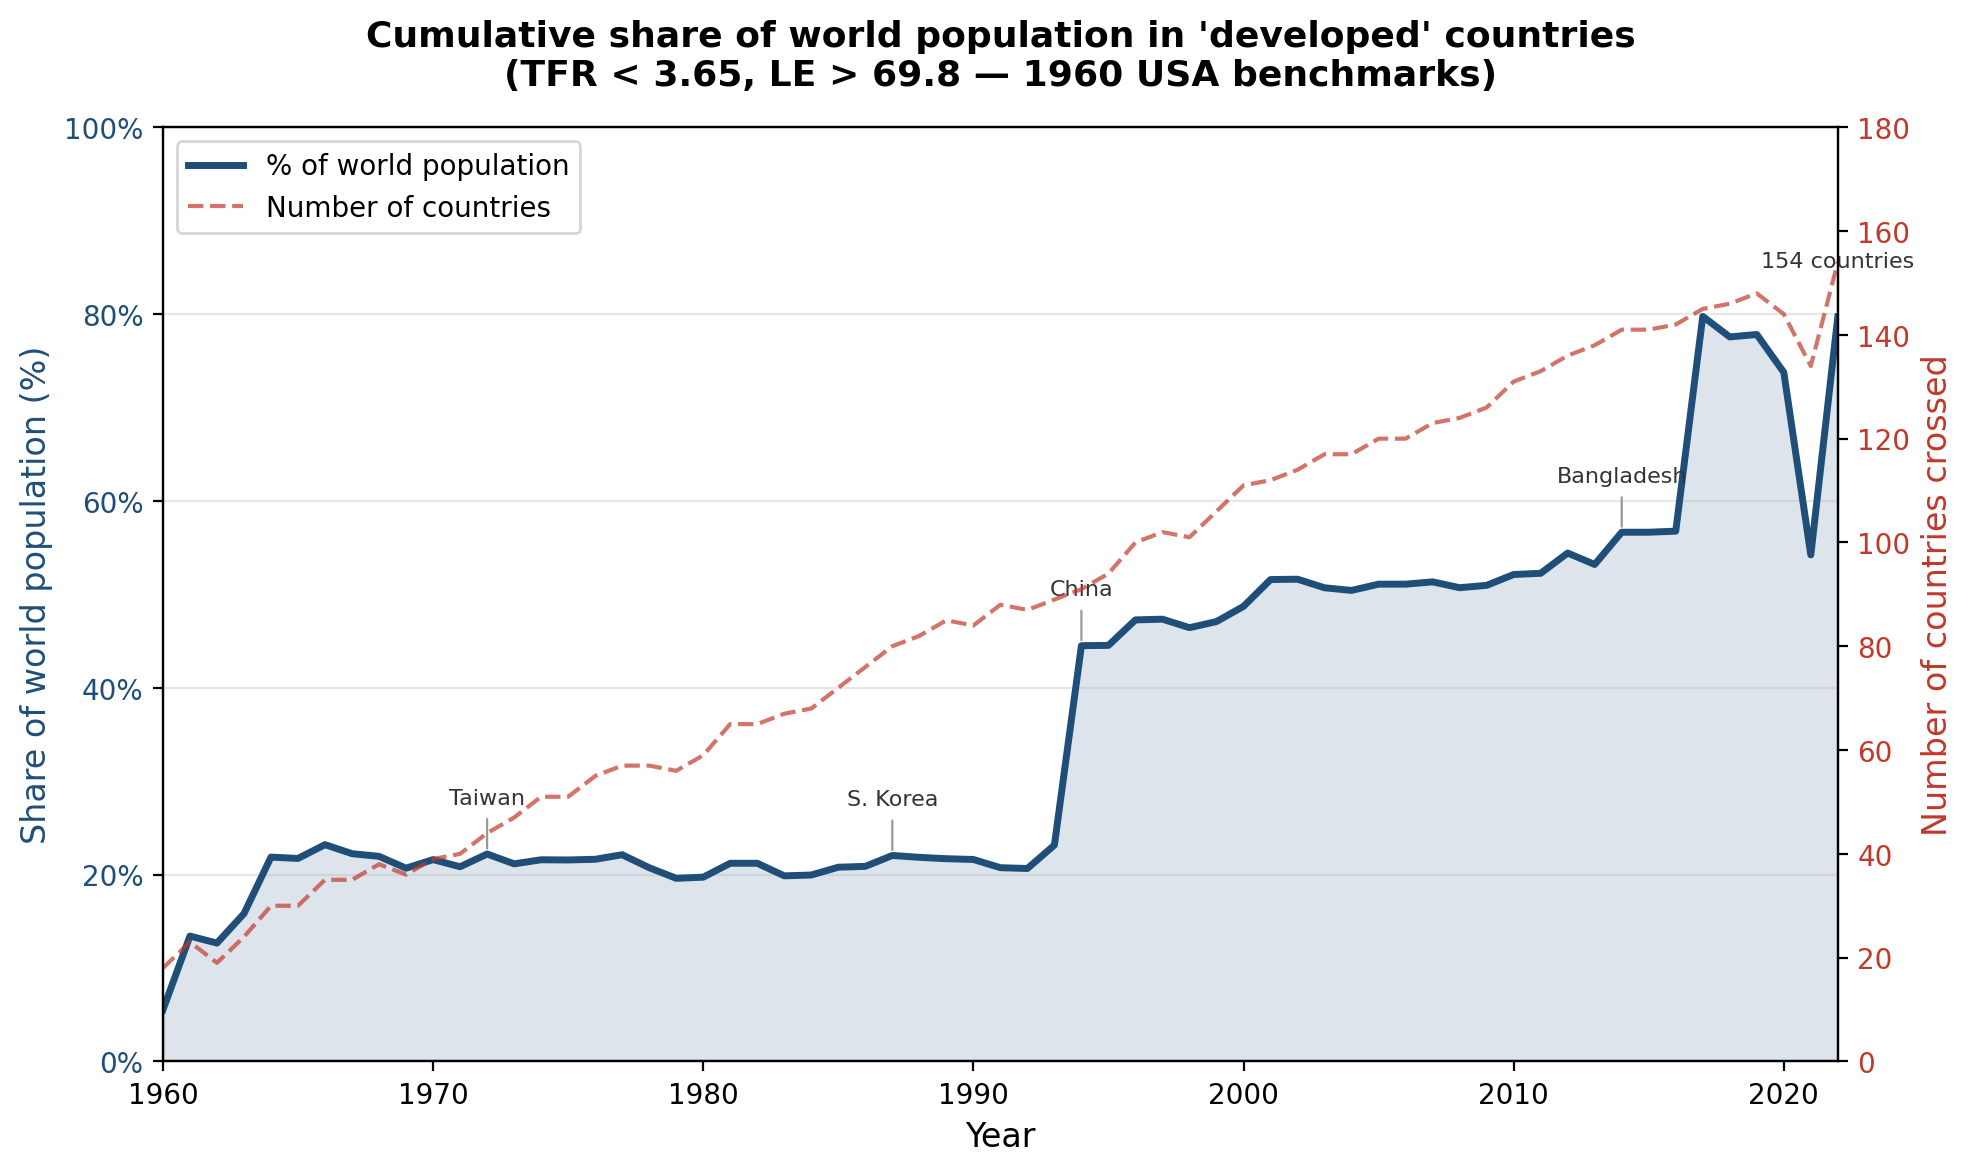
\includegraphics[width=\textwidth]{fig_cumulative_developed.png}
\caption{Cumulative share of world population crossing both
development thresholds (TFR \textless{} 3.65, LE \textgreater{} 69.8),
1960--2022. Slow climb from 13\% (1961) to \textasciitilde20\% (1993);
vertical jump in 1994 when China crosses; 50\% by 2001; 80\% by
2017--2022. \emph{(Source: World Bank WDI, WCDE v3. See
\texttt{scripts/fig\_cumulative\_developed.py})}}
\label{fig:1}
\end{figure}

\section{Theoretical Framework}\label{theoretical-framework}

\subsection{Easterlin's Founding Argument}\label{easterlins-founding-argument}

The education-first account of development has a precise starting point.
Easterlin (1981), in ``Why Isn't the Whole World Developed?'', asked why
modern economic growth had failed to diffuse uniformly given the
post-war availability of production technology. His answer was specific:
the binding constraint was the absence of mass schooling systems.
Technology transfers when it encounters a literate, numerate population
capable of deploying it. Without that population, it does not transfer,
regardless of capital access or external assistance.

Easterlin located this empirically in the historical spread of education
systems. The divergence in economic growth between early and late
industrializers tracked the divergence in mass schooling --- driven
originally by the Protestant Reformation's insistence on personal
scripture-reading, which produced mass literacy as a side-effect of
religious practice across Northern Europe. The distribution of
development in 1960 was substantially the distribution of schooling in
1860. Goldin \& Katz (2008) provide the most thorough historical
documentation of this transmission for the United States: the US ``human
capital century'' of 1910--1940, driven by the high school movement,
explains the majority of twentieth-century income growth --- a
within-country longitudinal result consistent with the cross-country
generational mechanism estimated here.

\subsection{Lutz and the Preston Curve}\label{lutz-and-the-preston-curve}

Lutz \& Kebede (2018) take Easterlin's historical argument into the
data. They reinterpret the Preston Curve (Preston 1975) --- the positive
relationship between national income and life expectancy --- by
replacing income with education on the x-axis. Three findings emerge.
First, the education--life expectancy relationship is tighter than the
income--life expectancy relationship. Second, and more important, the
upward shift of the curve over time --- the fact that populations live
longer today at the same income levels than in 1960 --- disappears when
education is on the x-axis (except at the lowest education level,
explained below). The ``wealth buys health'' reading of the Preston
Curve is an education story that income was proxying for, because income
and education are correlated but income is downstream of education in
the causal chain (Lutz 2009).

Third, and directly relevant to the scope of educational investment: the
education--life expectancy relationship shows no diminishing returns at
higher education levels. Unlike income, which follows the classic
concave Preston shape, the education curve remains approximately linear
from primary through tertiary. Lutz attributes this to a cognitive
mechanism: education changes the brain's capacity for planning, learning
from mistakes, and health-oriented decision-making across the entire
life course, and these gains accumulate at all levels of schooling. The
implication is that the case for educational investment does not weaken
as countries progress toward universal secondary; pushing further into
upper secondary and tertiary produces continued life expectancy gains.
This is consistent with the WCDE panel: among 70 countries with
lower-secondary completion above 85\% in 2010, college completion
carries a within-group correlation of r=0.44 with life expectancy. Mean
life expectancy rises from 73.5 years in the lowest college-completion
quartile to 79.0 years in the highest --- a 5.5-year gradient among
countries that have already solved the lower-secondary problem
(see \texttt{scripts/verify\_college\_le\_gradient.py}).

Deaton (2013) attributes the curve's upward shift to global health
technology diffusion independent of education. But health technology was
created by educated populations and its differential uptake tracks
education; Deaton's account does not identify an independent mechanism
(Section 5.3). If health technology diffusion were an independent
channel, countries with comparable access to the same global health
infrastructure would show comparable outcomes regardless of education
level. They do not. Vaccines, antibiotics, and oral rehydration
protocols are cheap, well-understood, and globally available --- the
technology has diffused. But a vaccine in a warehouse is not a
vaccinated child. Between the existence of a technology and its uptake
sits every household decision this paper describes: whether a mother
recognises symptoms, follows the protocol, spaces pregnancies, takes her
child to the clinic. The technology is globally available; the capacity
to convert it into behaviour is locally determined by education. The
existence of diffusion \emph{without} uniform outcomes is itself
evidence that education is the operative variable.

Lutz \& Kebede (2018) document one further finding: life expectancy at
the lowest education level in 2010 \emph{exceeds} the 1970 baseline for
that same level. This is the only level at which a genuine upward
Preston Curve shift remains when education replaces income on the
x-axis. The residual is education-mediated provision operating through
international institutions: educated actors produced vaccines,
antibiotics, and oral rehydration protocols; educated supply chains
distributed them to the populations with the lowest educational bases.
Sen's ``support-led security'' in its MDG-era form is not evidence that
provision works without education. It is evidence that a sufficiently
educated global class can deliver welfare externally to populations
still building their own educational base --- temporarily and without
accumulating.

\subsection{The Generational Transmission Mechanism: PT and Agency}\label{the-generational-transmission-mechanism-pt-and-agency}

The mechanism connecting these observations is generational
transmission. \textbf{PT (Parental Transmission)} is cultural
transmission from parent to child. The channel is biological, but what
travels through it is cultural. The paper measures PT through education
completion because that is the measurable proxy; what parents actually
transmit is broader --- norms, aspirations, health behaviours, the
decision to send the next child to school. PT is the base unit. It
transmits across generations: the grandchild's attainment reflects the
grandparent's through two sequential cycles (\textasciitilde50 years),
the great-grandchild's through three (\textasciitilde75 years).

PT explains persistence --- why educational gains never depreciate. But
persistence alone does not produce development outcomes. \textbf{Agency}
does: the categorical reorganisation of the brain that formal education
produces (Section 5.2) expresses itself across a lifetime of household
decisions --- fertility, health, investment, and children's schooling. The \textasciitilde25-year
lag between educational investment and development outcomes is the
interval for educated children to become adults exercising these
decisions. Taiwan's development crossing arrived \textasciitilde20 years
after educational expansion began: one generation of agency. Kerala's
arrived at \textasciitilde65 years: three generations of slow
accumulation before enough of the population was educated for agency to
produce population-level development outcomes. The variation in lag
length follows from biology, not assumption: a woman completing lower
secondary at age 15--18 has children reaching school age 20--30 years
later.
Educational expansion has two parts. PT provides durability: it
transmits what parents already have. State investment provides reach: it
brings first-generation learners into the system and lifts the level
beyond what parents alone would transmit. Where the state invests, both
channels operate together --- parents transmit what they have while the
state reaches children whose parents have nothing (Section 6.1). Where
the state does not invest, PT alone preserves what the parent already
has --- nearly perfectly, but nothing more.

The variation across countries is not a taxonomy of distinct mechanisms
but three speeds of the same one. \textbf{PT alone} is the baseline: a
parent transmits what they have, the next generation does the same.
Without state investment, this is the only channel --- century-scale, as
in pre-modern Europe, which took 100--150 years to complete the S-curve.
\textbf{Competing priority}: the state builds schools, but education
competes with health, nutrition, security, and governance for funding
and political attention. Multi-generational, as in India and most
post-colonial countries. \textbf{Singular priority}: the state makes
education the unconditional national focus, building ahead of need.
One-generation crossing --- Korea, Singapore, Cuba, Meiji Japan. All
three are education-mediated. What varies is how the state allocates
above the PT baseline: dispersed or concentrated.

PT's durability is not a statistical curiosity --- it reflects a
biological channel. Humans have plastic brains, but plasticity alone
explains nothing: a plastic brain in isolation learns nothing useful.
What delivers knowledge to the plastic brain is the human juvenile
dependency period --- roughly 18 years, compared to 8 for chimpanzees,
the longest in any species (Konner 2010). A dedicated learner embedded
with a dedicated teacher for nearly two decades: long enough for
cumulative cultural knowledge to be absorbed deeply enough to become the
learner's own baseline. The learner then becomes the teacher.
Plasticity is the hardware; the extended dependency is the protocol; the
parent is the carrier (Boyd \& Richerson 1985). The channel is biological
in the sense that it requires the species-specific parent-child
dependency period, not in the sense of genetic transmission --- what
travels through it is cultural knowledge, not DNA.

This architecture explains three properties. Non-depreciation: 18 years
of sustained transmission consolidates knowledge so deeply that it
persists for life. Formal education is the most powerful payload ever
delivered through this channel. Amplification: when the state builds
schools, it loads additional knowledge onto the same channel --- the
$\beta > 1$ result (Section 6.1). Catastrophic reset: because the
knowledge lives in the teacher, not the institution, destroying the
educated population leaves the next generation's plastic brains with
nothing to absorb. Cambodia (Section 7.1) is this test: schools rebuilt
within a decade, progress stalled for a generation. Knox did not invent
parental transmission; he institutionalised it, channelling formal
schooling through a mechanism as old as the species.

\subsection{From Action to Talk: How Education Reaches Beyond the Household}\label{from-action-to-talk-how-education-reaches-beyond-the-household}

The PT mechanism operates through action --- the household decisions of
educated adults. But education's effects extend beyond the household,
and the nature of that extension changes as the radius widens. Two
things widen it simultaneously. First, education expands the boundary of
who counts as ``my people'' --- literacy connects you to people you have
never met, shared knowledge creates shared identity, coalitional
psychology (Tooby \& Cosmides 2010) allows flexible group boundaries
that education stretches from kin to region to nation. Second, education
releases surplus: educated parents have fewer children and nearly all
survive, freeing time, money, and attention that a parent with seven
children and three surviving does not have. The arc widens (who you
invest in) and the constraint loosens (what you can invest). Neither
alone is sufficient. Surplus without expanded identity stays within the
family --- wealth hoarding, dynasty-building. Expanded identity without
surplus is talk with no resources behind it.

At the \textbf{household}, education is action. The parent raises the
child, recognises symptoms, spaces births, sends the next child to
school. The 18-year biological channel guarantees delivery. There is no
choice to disperse --- you educate the child in front of you. PT fires
automatically; gains compound into the next generation.

At the \textbf{kin and identity} radius, education is still action but
identity-directed. Siblings tutor younger siblings --- strongest during
early transition, high fertility, low parental base. Extended family
members in multigenerational households (South Asia, sub-Saharan Africa,
East Asia) transmit educational norms at timescales shorter than the
nuclear PT interval. Diaspora invest back in home communities ---
educated Keralites in the Gulf funding schools in Thrissur, Indian
professionals abroad channelling resources to home states. The boundary
between kin and non-kin is blurred: Hamilton's kin-preferential
investment shades into coalitional identity defined by caste, region,
ethnicity, and nationality. The investment is concrete, directed, and
still compounding.

Beyond identity, education becomes \textbf{talk}: advocacy, normative
pressure, policy campaigns, global health delivery. The actor has no
identity stake. The consequences are real --- outcomes get measured, aid
gets redirected, the MDGs and SDGs track progress --- but diluted across
every good cause simultaneously. This is where competing priorities
emerge. At the household level there is no competition: you educate your
child. At the identity level the investment is still directed. It is
only when educated advocates operate beyond identity that they disperse
across health AND nutrition AND governance AND education simultaneously
--- the competing-priority pathway (Section 3.3) that explains why most
countries expand slowly. Global concern --- educated actors delivering
welfare technology to populations with no identity connection --- is kin
relaxation at its widest: the boundary has expanded to include
strangers, and the surplus exists to act on it.

The critical distinction is durability. Investment at the household and
kin radii compounds into the next generation through PT. Identity-level
investment builds institutions that persist beyond any individual donor.
But externally delivered non-education interventions at the global radius
--- vaccines, nutrition programmes, oral rehydration --- are durable
only as long as the institutions maintaining them remain engaged.
Non-education intervention buys time; educational investment changes
trajectory. This is also the mechanism behind the global educational
expansion that year fixed effects absorb (Section 5.3): domestic demand,
international advocacy, and normative pressure from educated populations
all contribute to a global education signal whose components need not be
disentangled for the causal claim to hold.

The in-group/out-group boundary is the same mechanism running in
reverse. Violence and exclusion toward out-groups is the primate
default --- the tight boundary that directs investment inward and
hostility outward. In a zero-sum world, hierarchy suppresses mass
education rationally: educating the out-group threatens the in-group's
position. The surface vocabularies change across eras and cultures; the
underlying structure does not. What education does is relax this
boundary. As the in-group expands --- through shared literacy, shared
institutions, children in the same schools --- the out-group shrinks.
Mass education dissolves the boundary at scale: once everyone's children
are in the system, the out-group category empties. The failure mode that
remains is not exclusion but dilution --- educated advocates dispersing
across every good cause instead of concentrating on the one that
compounds. The dilution is structurally difficult to correct. Educated people
consistently rate education as important --- but ``important'' means one
of many important things, ranked alongside health, nutrition, governance,
and security. They cannot categorise it as \emph{fundamental} --- the
one input without which the others do not operate --- because that would
require seeing their own cognition from outside: recognising that the
capacity to evaluate, compare, and advocate is itself the product of
education. Uneducated people cannot see the value of formal education
because they have not experienced it. The people who could identify
education as fundamental cannot, because they are inside it; the people
who would benefit most cannot, because they are outside it. The
historical exceptions confirm the rule: Knox acted from religious
conviction, Meiji Japan from existential military threat, Korea from
Cold War survival. In every case where the decisive commitment was made,
the motivation was not developmental --- it came from outside the
development frame entirely. No one broke through the invisibility by
seeing education more clearly; they broke through by not looking at
development at all.

The theory predicts that education's predictive power should decay
smoothly across lag lengths, not in discrete 25-year pulses --- because
real populations have continuous age structure. People are of all ages
at all times. Educational investment enters the population continuously
as successive cohorts complete schooling, and agency --- the household
decisions that produce development outcomes --- is exercised by adults
across their entire lifetimes. Figure 3 (Section 6.2) confirms this:
gradual decay across lags 0--100, the signature of a continuous
process rather than discrete generational cycles overlapping.

\subsection{Demographic Structure and Resilience}\label{demographic-structure-and-resilience}

The accumulation has a demographic structure that varies with the level
of completion. Fertility declines continuously as female secondary
completion rises. The biological mechanism is a shift in reproductive
strategy, not an override of the reproductive drive: in high-mortality
environments, the optimal strategy is quantity --- have many children
because some will die. Education changes both inputs to this calculus.
Child survival rises (fewer births needed to achieve the same number of
surviving children), and the planning horizon extends --- a literate
parent can see that investing more in fewer children produces better
outcomes than hedging with numbers. The drive to maximise offspring
success is unchanged; what changes is the strategy that serves it.
Caldwell (1982) identified the reversal of intergenerational wealth
flows --- from children supporting parents to parents investing in
children --- as the trigger for fertility decline. But the steepest
fertility decline occurs at primary education (R²=0.65, Section 6.3),
where women are barely literate and not calculating investment returns
or wealth flows. What primary education gives is agency over
preferences that already exist --- the capacity to read a
contraceptive instruction, understand a health protocol, act on a
desire not to be pregnant continuously. Caldwell's wealth flow reversal
is at best a secondary/tertiary phenomenon; the first and largest
fertility decline happens before anyone is doing his calculus. Caldwell
also cannot explain why fertility continues falling past the point where
wealth constraints disappear: rich uneducated populations (Gulf states
pre-education expansion) had high fertility despite unlimited resources.
The variable is education, not wealth flows. The
steepest demographic headwinds are at the lowest completion levels,
where total fertility rates are typically above 4, population growth is
rapid, and the gains from each educated cohort are diluted across a
larger and faster-growing next generation. As completion rises, fertility
falls, child survival improves, and household resources per child
increase. The educational investment does
not accelerate at any particular threshold --- Korea's data shows steady
state-driven expansion from \textasciitilde25\% to over 90\% with no
inflection at any point (Figure 2). Sustained state investment is
required all the way to near-universal completion. Critically, PT is a
household mechanism. It operates through millions of individual family
decisions --- whether to send a daughter to secondary school, how many
children to have, whether to vaccinate, how to interpret health
information. States can create conditions for these decisions; they
cannot make them.

\subsection{How Education Produces Development}\label{how-education-produces-development}

Nutrition and physical security are not preconditions for educational
expansion --- they are consequences of it. The asymmetry operates in two
directions: (1) every successful educational expansion was made through
poor nutrition and insecurity, not after resolving them; (2) destroying
education causes multigenerational damage while destroying security does
not.

First, the historical baseline. Humans have lived at the margins of
subsistence nutrition for most of recorded history. This is not a recent
problem to be solved before educational investment can begin --- it is
the starting condition from which every successful educational expansion
was made. Korea in 1953 was a devastated post-war country with
widespread malnutrition. Japan in 1872 was a poor agrarian nation
operating at subsistence. Nepal in 1990 had GDP per capita of \$423 and
lower-secondary completion of just 27\%. Nutrition improved
\emph{because} education expanded --- through better agricultural
knowledge, health behaviours, and the income gains that educated
workforces generate. There is no historical example of a population that
improved nutrition first and then expanded education. The causal arrow
runs education → nutrition at the scale of national development, not the
reverse.

\medskip
Second, what destruction proves. Physical insecurity is not a
development-stopping condition --- conflict is episodic and localised,
and its frequency has declined as education has spread. Sri Lanka's
26-year civil war did not break the educational base --- conflict slowed
the LE crossing by roughly 12 years (Section 7), but development arrived
in 1993. Myanmar's continuous civil war since 1948 --- the world's
longest-running --- did not prevent TFR falling from 5.9 (1960) to 2.3
(2015) and LE rising from 44.1 to 65.3, all at GDP below \$1,200 (World
Bank WDI). Myanmar has crossed the TFR threshold but not the LE
threshold (65.3 vs 69.8). The asymmetry is diagnostic: TFR responds to
primary education, which Myanmar achieved; LE requires lower secondary,
which conflict delayed. War takes life out of the individual's hands ---
violence kills in ways education cannot fully mediate --- but fertility decisions
remain in the individual's hands even during conflict. Across eight
major conflict episodes (Myanmar, Sri Lanka, Bosnia, Cambodia, Rwanda,
Colombia, Afghanistan), TFR never reversed during war, while LE dipped
in five of the eight. Sri Lanka shows the same pattern: TFR crossed
during the civil war (1983--2009), but LE stalled for two decades before
resuming its climb after the war ended.

Only the targeted destruction of the educated population itself ---
Cambodia (Section 7.1) --- resets the generational clock. Security loss
is a disturbance the mechanism runs through; education loss takes a
generation to repair because the parental baseline cannot be rebuilt
from buildings alone. The contrast with Uganda (Section 4) confirms: the
binding constraint is the educational foundation, not provision.


\section{Causal Identification: The Bad Control Problem and Natural Experiments}\label{causal-identification-the-bad-control-problem-and-natural-experiments}

Every model in this literature that controls for GDP commits what Pearl
(2009) calls the bad control error (see also Angrist \& Pischke 2009,
ch.~3): conditioning on a variable that is itself caused by the variable
of interest.

Education predicts GDP one generation forward (FE β=+0.012 log-points
per 1pp education gain; Table 2). In the pooled panel, GDP appears to
predict education forward at similar strength --- but this symmetry is
an artifact of averaging across all education levels. Restricting to
countries below 10\% completion, education predicts future child
education at R²=0.594 while GDP predicts future child education at
R²=0.290 --- a 2× asymmetry that widens to 3.4× at the 30\% cutoff
(Section 6.2). The causal argument rests on this asymmetry, on
durability (Figure 3), and on the parental income channel collapsing in
magnitude once parental education is controlled. Including current GDP
as a control blocks part of the education signal through the income
channel. The result is a biased downward estimate of education's true
effect.

My primary analysis excludes GDP from the policy residual --- the
difference between actual and predicted education outcomes --- for
precisely this reason. The residual measures education delivered above
the generational baseline, without crediting any achievement to the
income that education itself generated.

Without an educational foundation, development gains reverse. Uganda in
1960 had identical life expectancy to India (both 45.6); by 1965, Uganda
had pulled ahead (48.3 vs 45.6) --- health investment without
educational investment produced early gains. But those gains could not
sustain themselves. By 1975, India had crossed Uganda; by 1984, India
was 12 years ahead. By 1980, Uganda's life expectancy had fallen to 43.5
--- below its 1960 level. The difference is not funding --- India's
health services were no better resourced. It is that India's educational
expansion, while slow, had been building a parental base that continued
to operate through household decisions. Uganda had no comparable
educational foundation; without it, the health gains reversed.

China is the comparison case: it had an educational foundation; Uganda
did not. China crossed the LE threshold (Section 7). Uganda has not
arrived after 65 years.

A note on causal identification is warranted before presenting this
evidence. The canonical approach to identifying education effects is
instrumental variables: Duflo (2001) exploits variation in school
construction across Indonesian districts to identify the causal effect
of education on individual earnings. Duflo's design works because the
instrument varies education exposure at short-run individual timescales
--- the relevant lag between schooling and earnings is five to fifteen
years. At 25-year generational
timescales across 187 countries, the identification strategy is
necessarily different --- and stronger. It rests on three identification
structures. First, temporal ordering: parental cohort precedes child
cohort by biological necessity, ruling out reverse causality at the
individual level. Second, the lag-decay shape (Figure 3; Section 6.2):
education and income produce structurally different decay profiles that
autocorrelation cannot explain. Third, and most directly, a battery of
natural experiments --- cases where parental education was exogenously
disrupted or where other development inputs were removed while education
persisted --- produce outcomes that pure autocorrelation cannot predict.
The battery includes: Cambodia (population destruction → generational
shadow); Uganda vs India (education destruction vs thin base → divergent
recovery); Sri Lanka (civil war, PT unbroken, development on schedule);
Myanmar (73 years of conflict, outcomes moved on schedule); China
(barefoot doctors dismantled, LE continued rising); Korea vs Philippines
(identical colonial base, divergent state commitment); and the Asian
Financial Crisis (income wiped, education untouched). The cases are
developed in Sections 7 and 9. Cambodia --- the most direct available
test of PT --- is presented in Section 7 alongside the other case
studies, where the WCDE data it relies on has been introduced.


\section{Data and Empirical Strategy}\label{data-and-empirical-strategy}

\subsection{Data}\label{data}

Education data are from WCDE v3 (Lutz et al.~2021): lower secondary
completion rates for the 20--24 age cohort, both sexes, which reflects
completed education rather than enrolment. All education percentages in
this paper refer to this measure unless otherwise noted. Coverage: 187
countries, 1950--2015 at five-year intervals; the core generational
panel uses 1975--2015 (1,683 country-years); the residualization
analysis (Section 6.3) extends to T=1960--1990 with education
interpolated to annual values for precise threshold identification.
Long-run analysis uses a 28-country subsample extending back to 1900,
selected for data availability; the generational coefficient varies
systematically with baseline education level (Section 6.1). GDP data:
World Bank, constant 2017 USD, per capita, log-transformed. Life
expectancy, TFR, and under-5 mortality: World Bank WDI. Parental
education: each country's lower secondary completion lagged 25 years
(T−25).

\subsection{Completion as the Operative Variable}\label{completion-as-the-operative-variable}

The quality objection --- that completion measures quantity rather than
quality (Hanushek \& Woessmann 2008, 2015) --- applies to a different
question. Hanushek \& Woessmann's dataset begins in 1960 and spans
roughly 40 years; their test score measures do not exist before
international assessments began in the 1960s. The educational expansions
that explain Korea, Taiwan, Sri Lanka, and Kerala all precede their
data. More fundamentally, quality follows quantity in the historical
sequence: a literate, numerate population is the precondition for any
test to be administered. WCDE completion is the appropriate measure for
a 50--100 year generational mechanism; Hanushek \& Woessmann's quality
measures capture downstream returns to education already achieved.

The quality objection also misidentifies what PT transmits. Formal
education --- even at the lowest quality --- represents a categorical
discontinuity from oral cultural transmission. The neuroscience is
unambiguous: literacy physically restructures the brain's visual
processing pathways (Dehaene et al.~2010), and numeracy recruits
parietal circuits unavailable to innumerate populations (Gordon 2004;
Frank et al.~2008). These are not marginal improvements on existing
capacities --- they are new cognitive technologies that do not develop
without schooling, regardless of intelligence or environment. A stunted
child who learns to read undergoes the same categorical
reorganisation as a well-nourished one; the stunting reduces efficiency
but does not eliminate the discontinuity. The distance from no formal
education to any formal education is categorical; the distance from a
bad school to a good school is marginal by comparison. PT fires on this
categorical threshold --- the household decision to send the next
generation to school, the health and fertility behaviours that change
with any education, the aspirational shift that follows. The
transmission is triggered by exposure, not by test scores. The endemic
disease and malnutrition objections make the same error: they ask
whether disease or hunger reduces cognitive performance, when the
operative variable is whether the child was in school at all.

\subsection{Empirical Strategy}\label{empirical-strategy}

Primary specification --- country fixed effects regression:

\[E_{it} = \alpha_i + \beta_1 E_{i,t-25} + \varepsilon_{it}\]

where \(E_{it}\) is education completion in country \(i\) at time \(t\),
\(E_{i,t-25}\) is the same country's completion 25 years earlier
(parental cohort), and \(\alpha_i\) absorbs all time-invariant country
characteristics including institutions, geography, culture, and colonial
history. The coefficient is identified entirely from within-country
variation over time.

Comparison specifications:

\[E_{it} = \alpha_i + \beta_2 \ln Y_{it} + \varepsilon_{it}\]

\[E_{it} = \alpha_i + \beta_1 E_{i,t-25} + \beta_2 \ln Y_{it} + \varepsilon_{it}\]

For development outcomes, forward-lagged by one generation
(\textasciitilde25 years) to eliminate reverse causality:

\[O_{i,t+25} = \alpha_i + \gamma_1 E_{it} + \gamma_2 O_{it} + \varepsilon_{it}\]

where \(O_{it}\) controls for initial outcome levels. \(O_{it}\) is not
a bad control in the Pearl (2009) sense: it is caused by \emph{prior}
education (\(E_{i,t-25}\), the parental cohort), not by \(E_{it}\)
itself --- the generational mechanism means \(E_{it}\) has not yet had
time to affect \(O_{it}\). Conditioning on initial outcomes is
conservative; it absorbs prior trajectory and makes \(\gamma_1\) a lower
bound on education's true effect.

\textbf{Choice of education variable.} The main analysis uses aggregate
(both-sexes) lower secondary completion. Female completion produces
stronger R² on every outcome tested (Section 6.3). The aggregate
specification is retained as the more conservative test: if education
predicts development outcomes and GDP does not using the weaker
predictor, the claim holds a fortiori with the stronger one.

\textbf{Residualization strategy.} The comparison between education and
GDP as predictors is confounded by the fact that education drives GDP
growth. Countries develop serially: education rises first, GDP follows a
generation later. To isolate GDP's \emph{independent} predictive power,
I residualize log GDP against education using country FE --- regressing
log GDP(T) on education(T) within countries, and extracting the
residual: the component of GDP that is \emph{not} explained by
education. This residual is then used to predict development outcomes at
T+25. If the residualized GDP R² approaches zero, GDP has no independent
effect --- its apparent predictive power was education flowing through
income. This two-step procedure (Frisch-Waugh-Lovell) is applied across
three education levels (primary, lower secondary, upper secondary), four
outcomes (life expectancy, TFR, child mortality, child education), and
multiple entry-cohort/ceiling specifications (see
\texttt{scripts/edu\_vs\_gdp\_residualized.py},
\texttt{scripts/edu\_vs\_gdp\_tfr\_residualized.py},
\texttt{scripts/edu\_vs\_gdp\_child\_edu\_residualized.py}).

\textbf{Entry-cohort design.} The cutoff-based sample definition (e.g.,
``countries below 30\% completion'') selects observations, not
countries. A country at 28\% in one period and 35\% in the next
contributes one observation inside the cutoff and one outside. This
loses the country's full development trajectory. I supplement the cutoff
analysis with an entry-cohort design: for each threshold (10\% to 90\%,
in 1\% increments), identify the first year each country crosses that
threshold, then include all observations from that point forward --- but
only while education remains below a ceiling (50\%--90\%). Education
data are interpolated from WCDE 5-year intervals to annual values
(linear) for precise threshold identification. This tracks countries
through their development trajectory while excluding high-education
observations that mechanically compress the education coefficient (see
\texttt{scripts/edu\_vs\_gdp\_entry\_ceiling.py}).

\textbf{On year fixed effects.} Year FEs absorb part of the education
signal, not a confounder. Adding year FE to the country FE specification
dramatically reduces the parental coefficient (Table A1; Section 6.1).
Education levels rose across nearly all countries simultaneously after
1975. If that global trend were an external confounder --- something
outside education driving all countries upward --- then removing it
would reveal the true, smaller effect. But the trend is itself
education-driven: educated populations advocate for educational
expansion globally (Section 3.4), and year FEs absorb this signal along
with any genuine confounders. Section 6.1 quantifies the absorption.


\section{Results}\label{results}

\subsection{Education vs.\ GDP as Predictors of Attainment}\label{education-vs-gdp-as-predictors-of-attainment}

Among countries where the expansion is still active --- parental
completion below 30\%, where most of the remaining 20\% of humanity sits
--- education R²=0.70 vs GDP R²=0.21. Education leads by 3.3×. GDP's R²
barely changes across cutoffs (0.21--0.29); education's jumps from 0.54
to 0.70. GDP has no S-curve structure --- its R² is flat across all
cutoffs. The 30\% cutoff is not selected for favourable results:
education leads GDP at every cutoff from 10\% to 90\%, with ratios
ranging from 1.4× to 3.3× (see
\texttt{scripts/education\_vs\_gdp\_by\_cutoff.py}).

\textbf{Table 1.} Country fixed effects regressions: child lower
secondary completion on parental education and log GDP per capita.
Countries with parental completion below 30\% (active expansion); 655
country-years, 111 countries.

\begin{longtable}[]{@{}llll@{}}
\toprule
Model & Parental edu β & Log GDP β & R² (within) \\
\midrule
\endhead
(1) FE: child \textasciitilde{} parent & \textbf{1.354***} & --- &
\textbf{0.699} \\
(2) FE: child \textasciitilde{} log GDP & --- & 13.668*** & 0.211 \\
\bottomrule
\end{longtable}

\emph{Standard errors clustered by country. *** p\textless0.001.
Ceiling countries excluded; including them mechanically compresses both
coefficients toward parity (Section 6.1). Education leads GDP at every
cutoff from 10\%--90\%
(\texttt{scripts/education\_vs\_gdp\_by\_cutoff.py}). Female completion
produces stronger R² on every outcome; the aggregate is the more
conservative specification. The gender gap in children's completion
collapses universally as parental education rises; above 50\% parental
completion, it reverses (WCDE v3).}

The decisive test is the shape across lags (Figure 3; Section 6.2).

Education levels rose across nearly all countries simultaneously after
1975. One objection is that this global trend inflates the parental
coefficient. Year fixed effects test this.

\textbf{Year fixed effects absorb education, not a confounder.} When
country and year fixed effects are both included, the parental
coefficient among countries below 30\% completion yields β=0.740 (t=5.5,
R²=0.345, n=790, 138 countries). Year FEs absorb roughly half the
coefficient (from 1.354 to 0.740). The question is what that absorbed
component represents. If the global trend were an external confounder
--- health technology diffusion, trade integration, or Cold War
competition driving both education and development simultaneously ---
then removing it should reveal a weaker true effect, and the pre-trend
period should produce a weaker coefficient still. The opposite is
observed: the all-country panel (1900--2015), which includes decades
before any common global trend, produces β=1.24 (with ceiling
observations above 90\% excluded; see below). The pre-trend coefficient
is \emph{stronger}, not weaker --- consistent with year FEs absorbing
part of the education signal rather than removing a confounder (Section
5.3). The remaining β=0.740 is entirely within-country, within-period
variation --- a country whose parents were more educated than other
countries at the same education level in the same year still produces
more educated children. On the pooled panel, the two-way FE collapses to
β=0.080 (Table A1).

\textbf{β exceeds unity at every cutoff --- the autocorrelation test.}
Mere autocorrelation of a slow-moving stock produces β ≤ 1 --- each
generation preserving what the prior had, nothing more. The data shows
β far above unity.
Across all countries in the WCDE with sufficient data (1900--2015), the
naïve fixed-effects β equals 1.05 --- but this is a misleading average.
It includes observations where parental completion is already above
90\%, where β mechanically approaches zero because there is no room to
grow. Including these ceiling observations drags the average toward
unity, creating the false impression that transmission merely preserves
rather than amplifies. Excluding observations where parental completion
exceeds 90\% yields β=1.24 (R²=0.778); below 50\%, β=1.82 (R²=0.804);
below 20\%, β=2.83 (R²=0.721). At every cutoff, β exceeds unity ---
gains amplify across generations because the state adds reach on top of
what households transmit. This is the decisive test against the
autocorrelation objection: mere autocorrelation of a slow-moving stock
produces β ≤ 1, never β = 2.83 (see
\texttt{scripts/beta\_by\_ceiling\_cutoff.py}). The decline from β=1.24
to β=0.49 in the post-1975 panel reflects the S-curve structure: the
post-1975 panel oversamples countries near ceiling.

\textbf{The S-curve within countries.} Within individual countries, β
varies systematically with baseline education level (Figure 2). The
United States shows β=1.9 when its baseline was 13\% (early 20th
century), declining to β=0.08 when its baseline reached 92\%. Korea
shows β=6.5 at 1\% baseline, declining through β=3.6, β=1.8, and β=0.2
as its baseline rose to 59\%. Taiwan follows a nearly identical
trajectory (β=5.1 at 1.2\%). The Philippines (Section 9) shows a flatter
curve: β=4.4 at 1.5\% declining more slowly to β=0.4 at 49\%. The
S-curve structure is robust across all countries with sufficient
historical depth. Bangladesh shows β≈2 throughout its observed
trajectory (1--18\% baseline), consistent with a country still in the
steep part of the S-curve. India follows a similar pattern at β≈1.6
through 28\% baseline.

\begin{figure}[htbp]
\centering
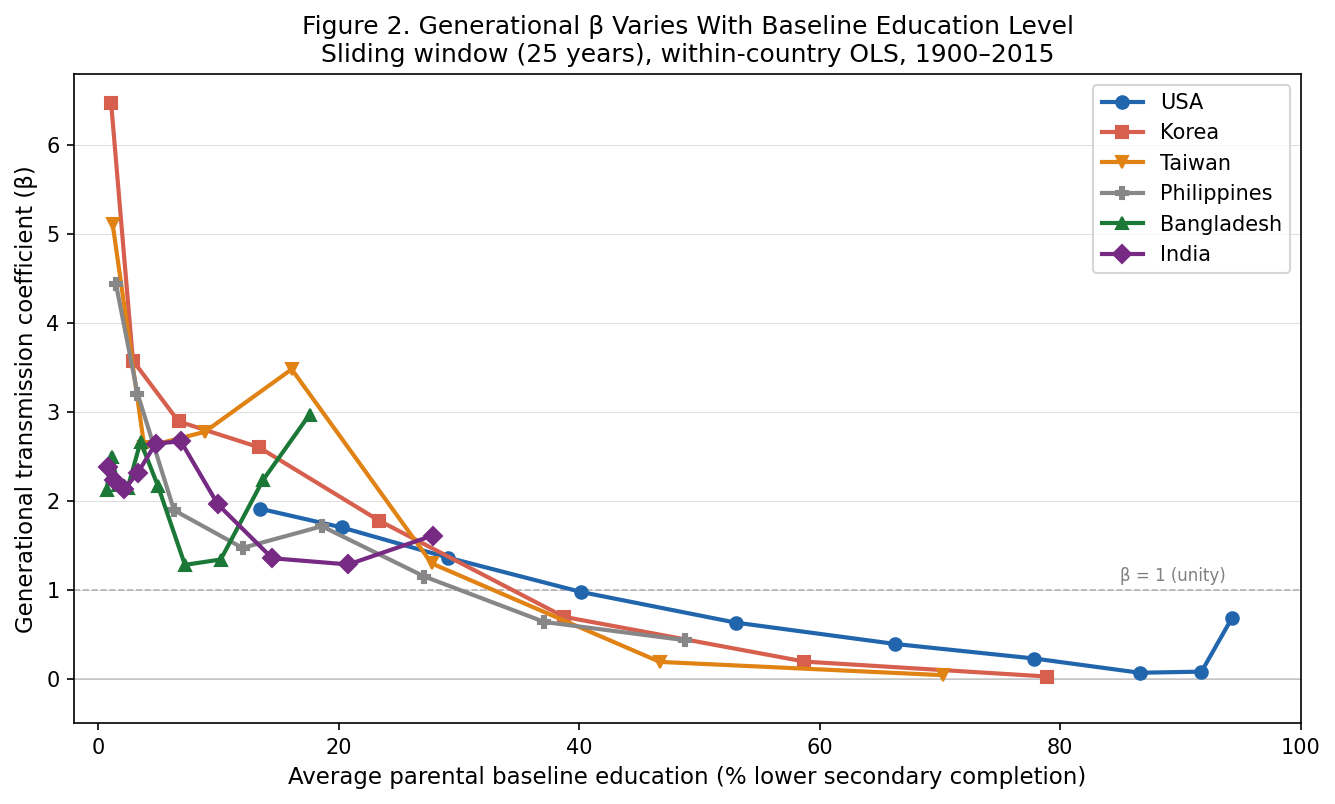
\includegraphics[width=\textwidth]{fig_beta_vs_baseline.png}
\caption{Generational $\beta$ varies systematically with baseline
education level. Each point represents a 25-year sliding window (6
child cohorts) within a single country, plotted against the average
parental baseline for that window. $\beta>1$ at low baselines
reflects state reach; $\beta\to0$ at high baselines reflects ceiling
compression. \emph{(Source: author's calculation, WCDE v3 long-run
cohort reconstruction 1875--2015 --- broader coverage than the
28-country regression panel in Table A3; Philippines historical data
carries greater uncertainty for pre-1950 colonial-era observations. See
\texttt{analysis/scripts/fig\_beta\_vs\_baseline.py})}}
\label{fig:2}
\end{figure}

The S-curve confirms the theoretical framework (Section 3.3).
β \textgreater{} 1 at low baselines is the empirical signature of state
reach --- the system expanding faster than household transmission alone.
β approaching zero at high baselines is ceiling compression, not
diminishing returns (distinct from Lutz \& Kebede's cross-level finding
that education's effect on life expectancy shows no diminishing returns
from primary through tertiary). The speed at which β collapses measures
how fast a country developed: Korea's β fell from 6.5 to near-zero in
60 years; the Philippines stretched the same range over 90 years;
Bangladesh's β has held at \textasciitilde2 for a century. Non-depreciation
holds universally --- the Cambodia test (Section 7.1).

Splitting the post-1975 panel by 1975 baseline confirms the S-curve
structure: countries below 20\% completion show β=1.585 (R²=0.706,
n=423, 47 countries), countries at 20--60\% show β=0.713 (R²=0.716,
n=675, 75 countries), and countries above 60\% show β=0.176 (R²=0.442,
n=585, 65 countries).

\subsection{Education Predicts Development Outcomes 25 Years Forward}\label{education-predicts-development-outcomes-25-years-forward}

\textbf{Table 2.} Fixed effects regressions: development outcomes one
generation forward (\textasciitilde25 years) on education, controlling
for initial outcomes. Panel A reports education predicting development
outcomes forward; Panel B reports the symmetric reverse regression (GDP
predicting education forward) to demonstrate mutual endogeneity.

\emph{Panel A: Education(T) → development outcomes(T+25)}

\begin{longtable}[]{@{}
  >{\raggedright\arraybackslash}p{(\columnwidth - 6\tabcolsep) * \real{0.2500}}
  >{\raggedright\arraybackslash}p{(\columnwidth - 6\tabcolsep) * \real{0.2500}}
  >{\raggedright\arraybackslash}p{(\columnwidth - 6\tabcolsep) * \real{0.2500}}
  >{\raggedright\arraybackslash}p{(\columnwidth - 6\tabcolsep) * \real{0.2500}}@{}}
\toprule
\begin{minipage}[b]{\linewidth}\raggedright
Outcome (one generation forward)
\end{minipage} & \begin{minipage}[b]{\linewidth}\raggedright
Education β
\end{minipage} & \begin{minipage}[b]{\linewidth}\raggedright
Initial outcome β
\end{minipage} & \begin{minipage}[b]{\linewidth}\raggedright
R² (within)
\end{minipage} \\
\midrule
\endhead
Log GDP per capita & +0.012*** & +0.173*** & 0.354 \\
Life expectancy (years) & +0.108*** & +0.301*** & 0.384 \\
Total fertility rate & −0.032*** & +0.037* & 0.367 \\
\bottomrule
\end{longtable}

The reverse regression tests whether GDP predicts future education
with comparable strength --- it does not once parental education is
controlled.

\emph{Panel B: Log GDP(T) → education(T+25) --- reverse regression}

\begin{longtable}[]{@{}
  >{\raggedright\arraybackslash}p{(\columnwidth - 6\tabcolsep) * \real{0.2500}}
  >{\raggedright\arraybackslash}p{(\columnwidth - 6\tabcolsep) * \real{0.2500}}
  >{\raggedright\arraybackslash}p{(\columnwidth - 6\tabcolsep) * \real{0.2500}}
  >{\raggedright\arraybackslash}p{(\columnwidth - 6\tabcolsep) * \real{0.2500}}@{}}
\toprule
\begin{minipage}[b]{\linewidth}\raggedright
Outcome (one generation forward)
\end{minipage} & \begin{minipage}[b]{\linewidth}\raggedright
Log GDP β
\end{minipage} & \begin{minipage}[b]{\linewidth}\raggedright
Initial edu β
\end{minipage} & \begin{minipage}[b]{\linewidth}\raggedright
R² (within)
\end{minipage} \\
\midrule
\endhead
Lower secondary completion & +14.85*** & --- & 0.272 \\
Lower secondary completion & +3.780*** & +0.485*** & 0.500 \\
\bottomrule
\end{longtable}

\emph{Country fixed effects, same panel. n=828 for GDP-education matched
obs.}

Each 1pp gain in lower secondary completion predicts, one generation
forward (\textasciitilde25 years): 1.2\% higher GDP per capita, 0.108
more years of life, and 0.032 fewer children per woman, identified from
within-country variation after controlling for initial conditions.

When education and income are each used to predict future child
education one generation forward, education dominates at every level.
Restricting to countries below 10\% completion --- where confounding
between the two variables is weakest --- education(T) predicts child
education(T+25) at R²=0.594 while GDP(T) predicts child education(T+25)
at R²=0.290 --- a 2× advantage. At the 30\% cutoff, the ratio widens to
3.4× (R²=0.701 vs 0.208, consistent with Table 1's 3.3×). At every
cutoff from 10\% to 90\%, education predicts future child education
better than GDP does (see
\texttt{scripts/education\_vs\_gdp\_by\_cutoff.py}).

The asymmetry is sharper still when the outcome is life expectancy.
Among countries below 30\% completion, education(T) predicts life
expectancy(T+25) at R²=0.309; GDP(T) predicts life expectancy(T+25) at
R²=0.021 --- education leads by 15× in the raw comparison. Among
countries below 10\% completion, education R²=0.628 while GDP R²=0.016
--- effectively zero. Education's R² remains stable at approximately
0.30 across all cutoffs; GDP's R² never exceeds 0.03. But even this
understates the asymmetry: as Section 6.3 shows, the small apparent
GDP signal vanishes entirely once education's contribution to GDP is
removed.

Figure 3 confirms this asymmetry across lag lengths. Measured across lag
lengths from 0 to 100 years, education and income have structurally
different decay profiles. Education's predictive power for life
expectancy decays slowly across three generational depths: R²=0.562 at
lag 0, R²=0.364 at lag 25, R²=0.171 at lag 50, R²=0.085 at lag 75.
Income's collapses within one generation --- already fading by lag
20--25. Beyond lag 50, income data does not thin out --- income itself
was uniformly low. Every pre-literate subsistence society sat at
approximately \$400--600 per capita (constant 2017 USD). This is not
missing data; it is the data: income had no cross-country variation
because education had not yet created it. Backfilling pre-1960 income at
\$500 per capita for all countries does not rescue income's predictive
power --- income's R² still collapses to zero by lag 60, while
education's remains positive at lag 100 (see
\texttt{scripts/backfill\_income\_lag\_test.py}). There is no hidden
income signal at long lags because there was no income variation to
predict with.

\begin{figure}[htbp]
\centering
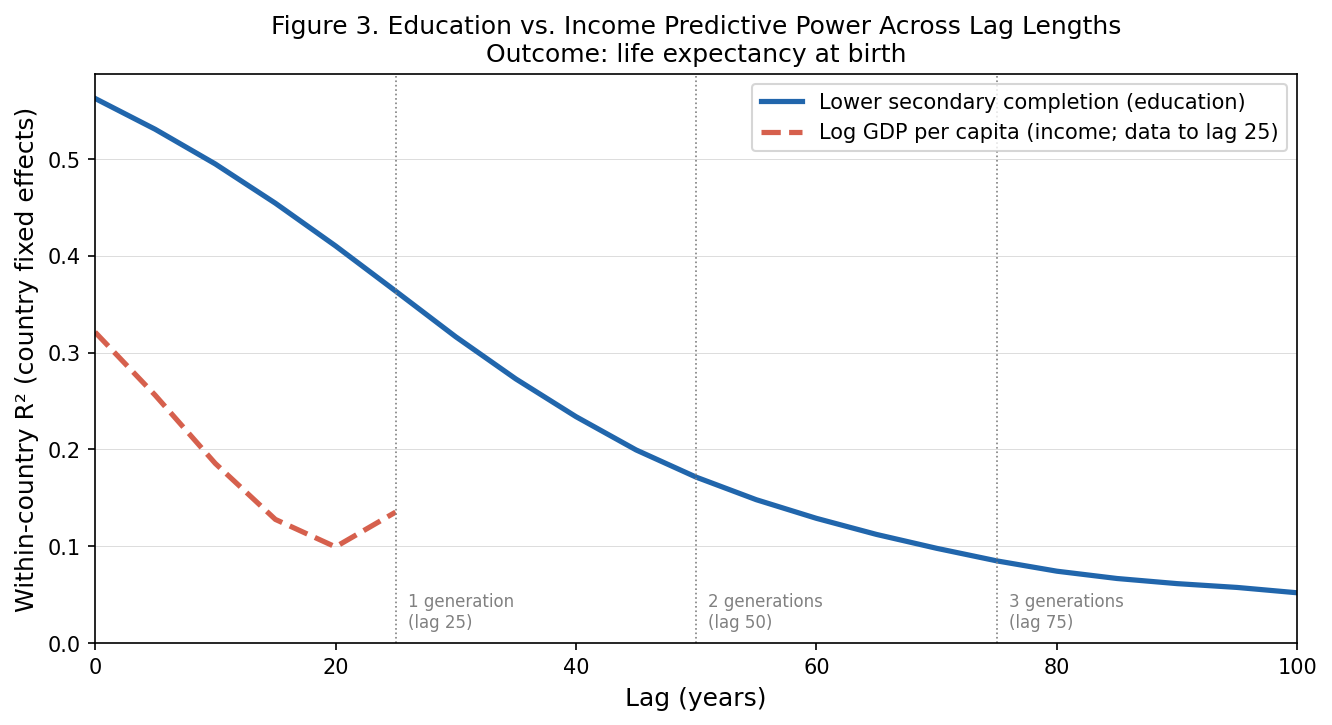
\includegraphics[width=\textwidth]{fig_lag_comparison.png}
\caption{Education vs.\ income predictive power across lag
lengths (within-country FE, outcome: life expectancy at birth).
Within-country $R^2$ for lower secondary completion and log GDP per capita
plotted against lag lengths from 0 to 100 years. Three generational
horizons marked (lag 25, 50, 75). Income shown through lag 25 only;
beyond that, income was uniformly low across pre-literate subsistence
societies. \emph{(Source: author's calculation, World Bank WDI and WCDE
v3. See \texttt{analysis/scripts/fig\_a1\_lag\_decay.py})}}
\label{fig:3}
\end{figure}

What lag 100 means in human terms: in countries that were still
expanding education, a great-grandparent's completion predicts how long
their great-grandchild will live --- four generations later. No other
development input has a comparable reach.

\subsection{GDP Has No Independent Effect}\label{gdp-has-no-independent-effect}

The comparison above overstates GDP's role. GDP(T) correlates with
future outcomes partly because education(T) drives GDP growth ---
countries develop serially. To test whether GDP has any
\emph{independent} predictive power, I residualize GDP against education
(Section 5.3) and use the residual --- the part of GDP not explained by
education --- to predict each outcome one generation forward.

\textbf{Table 2b.} Residualized GDP analysis: education vs.~raw GDP
vs.~GDP after removing education's contribution. Entry-cohort design
(entry ≥ 10\%, ceiling ≤ 90\%), country fixed effects, lower secondary
completion, T=1960--1990, lag=25 years.

\begin{longtable}[]{@{}
  >{\raggedright\arraybackslash}p{(\columnwidth - 10\tabcolsep) * \real{0.1667}}
  >{\raggedright\arraybackslash}p{(\columnwidth - 10\tabcolsep) * \real{0.1667}}
  >{\raggedright\arraybackslash}p{(\columnwidth - 10\tabcolsep) * \real{0.1667}}
  >{\raggedright\arraybackslash}p{(\columnwidth - 10\tabcolsep) * \real{0.1667}}
  >{\raggedright\arraybackslash}p{(\columnwidth - 10\tabcolsep) * \real{0.1667}}
  >{\raggedright\arraybackslash}p{(\columnwidth - 10\tabcolsep) * \real{0.1667}}@{}}
\toprule
\begin{minipage}[b]{\linewidth}\raggedright
Outcome (T+25)
\end{minipage} & \begin{minipage}[b]{\linewidth}\raggedright
Education R²
\end{minipage} & \begin{minipage}[b]{\linewidth}\raggedright
Raw GDP R²
\end{minipage} & \begin{minipage}[b]{\linewidth}\raggedright
Residualized GDP R²
\end{minipage} & \begin{minipage}[b]{\linewidth}\raggedright
p-value
\end{minipage} & \begin{minipage}[b]{\linewidth}\raggedright
Education → GDP R²
\end{minipage} \\
\midrule
\endhead
Life expectancy & 0.472 & 0.165 & \textbf{0.003} & 0.56 & 0.417 \\
Total fertility rate & 0.478 & 0.175 & \textbf{0.000} & 0.98 & 0.417 \\
Child education & 0.524 & 0.303 & \textbf{0.008} & 0.31 & 0.417 \\
Under-5 mortality & 0.284 & 0.046 & \textbf{0.023} & 0.11 & 0.417 \\
\bottomrule
\end{longtable}

\emph{Clustered standard errors by country. Residualized GDP R² reports
the within-R² of GDP residuals (orthogonal to education by construction)
predicting each outcome. Education → GDP R² reports how much of
within-country GDP variation is explained by education. See
\texttt{scripts/edu\_vs\_gdp\_residualized.py},
\texttt{scripts/edu\_vs\_gdp\_tfr\_residualized.py},
\texttt{scripts/edu\_vs\_gdp\_child\_edu\_residualized.py}.}

\begin{figure}[htbp]
\centering
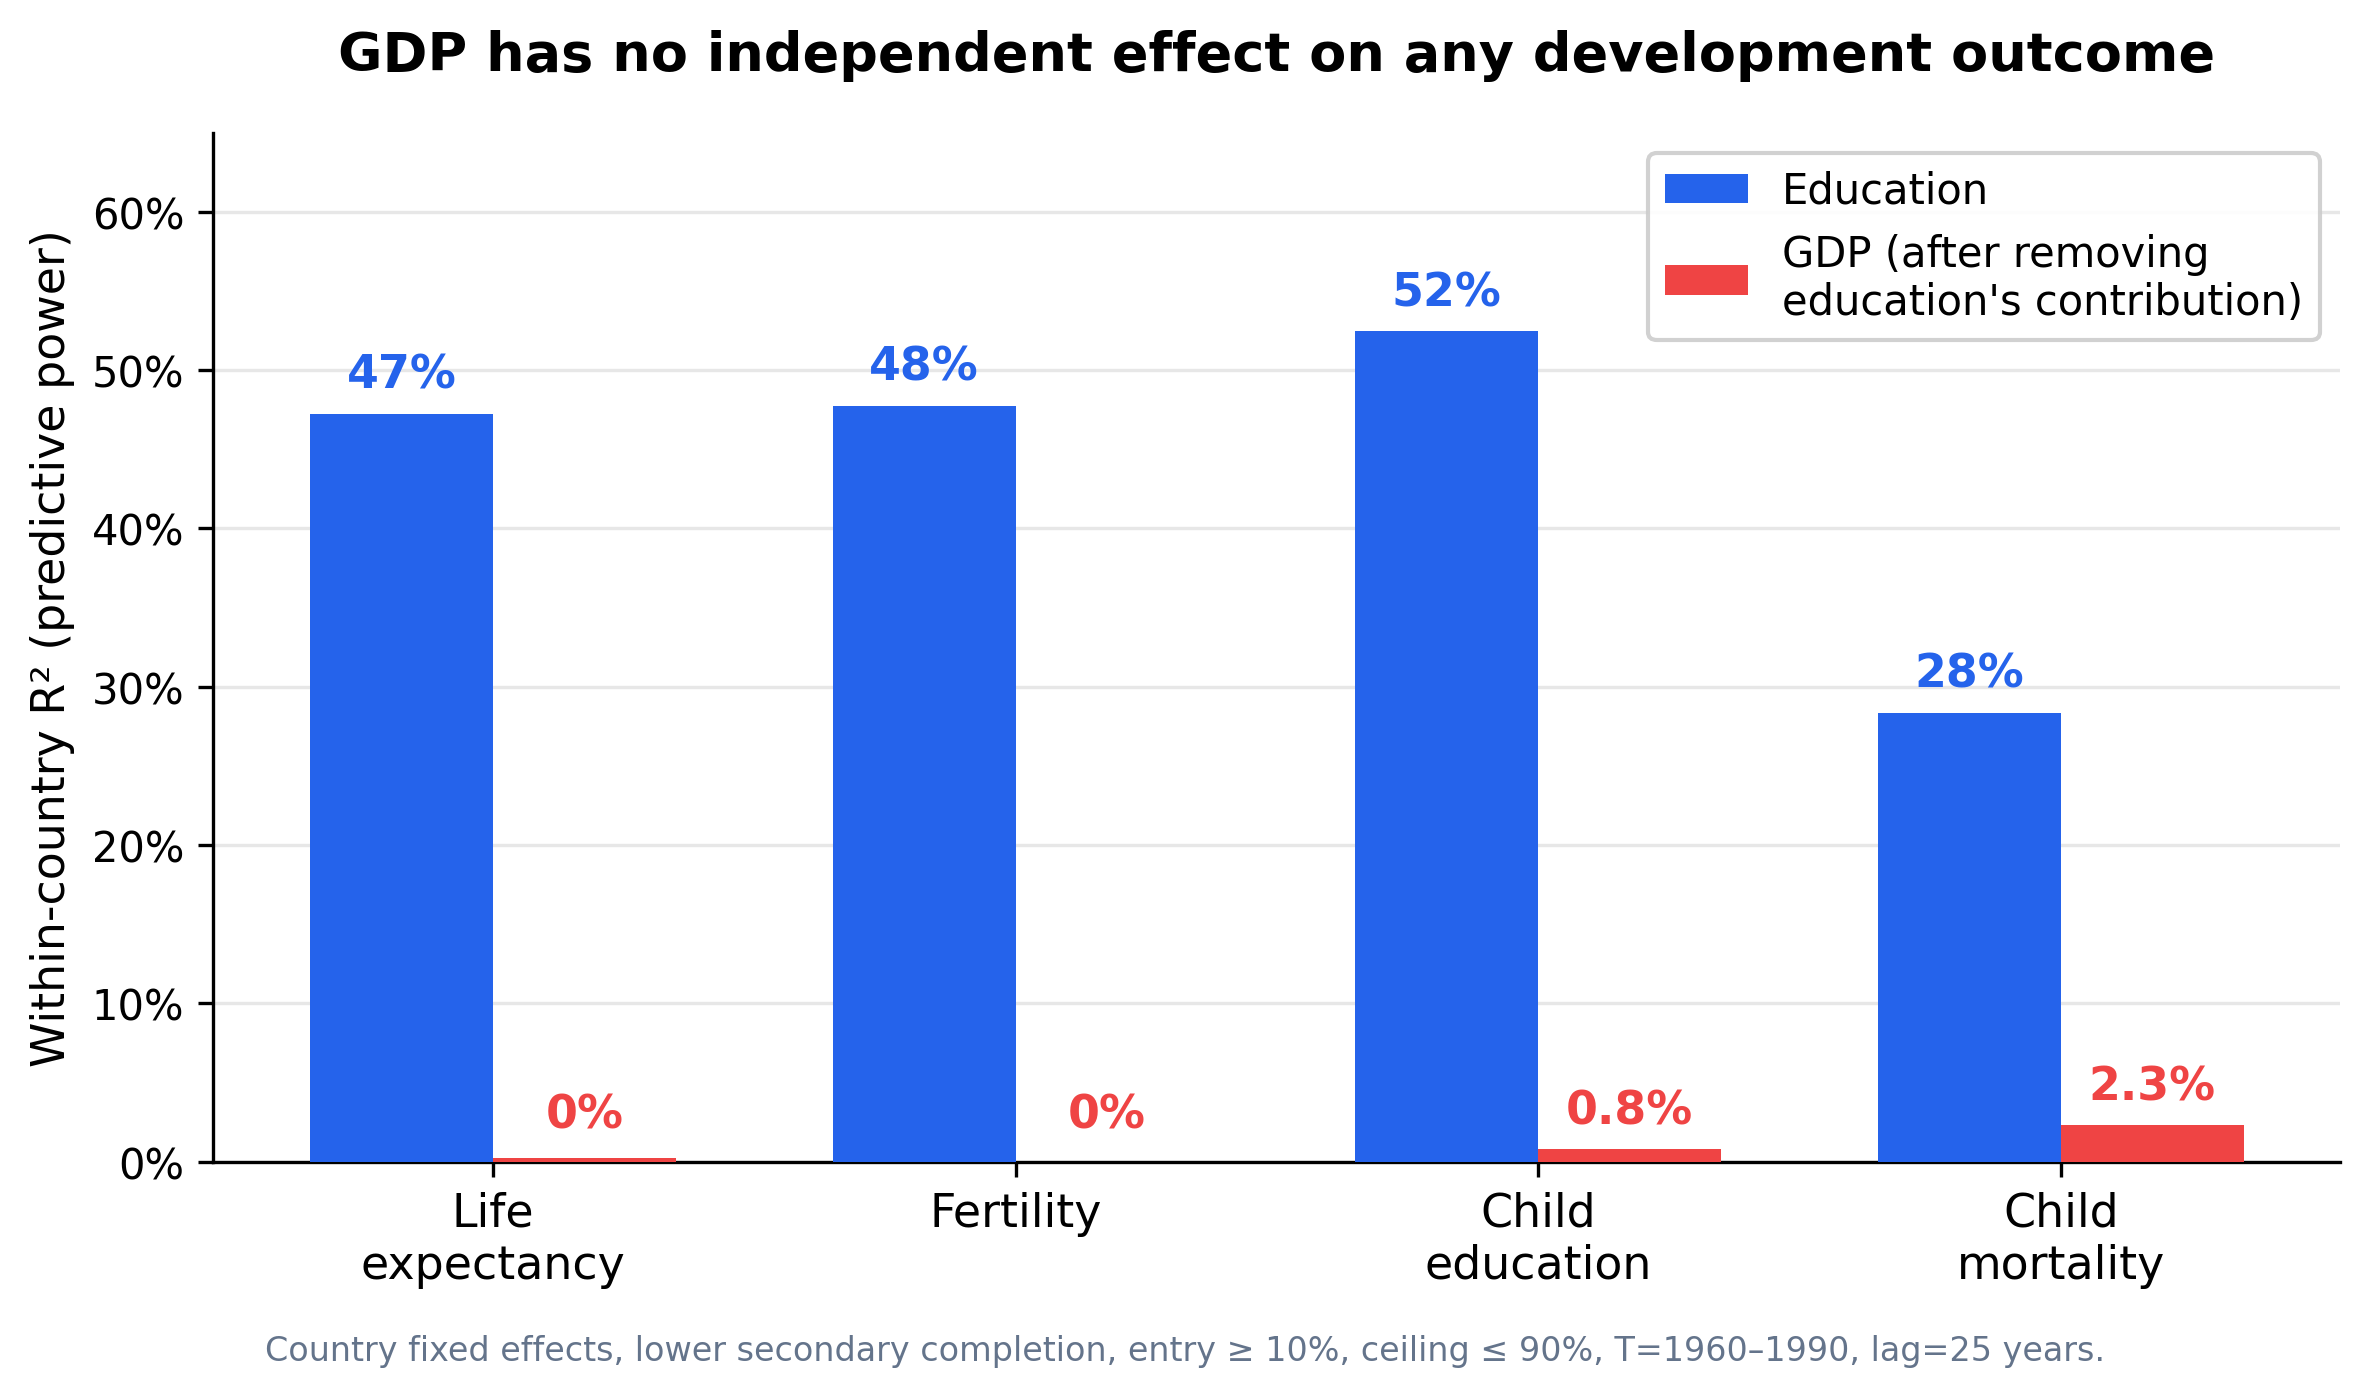
\includegraphics[width=\textwidth]{fig_residualization.png}
\caption{Education $R^2$ vs.\ residualized GDP $R^2$ across four
development outcomes. Blue: within-country $R^2$ for education predicting
each outcome one generation forward. Red: within-country $R^2$ for GDP
\emph{after removing education's contribution to GDP}. Entry-cohort
design (entry $\geq$ 10\%, ceiling $\leq$ 90\%), country fixed effects, lower
secondary completion, T=1960--1990, lag=25 years. \emph{(Source:
author's calculation. See \texttt{scripts/fig\_residualization.py})}}
\label{fig:4}
\end{figure}

The result is unambiguous: after removing education's contribution to
GDP, income has no independent predictive power for any development
outcome. The residualized GDP R² never exceeds 0.023, and the associated
p-values are all above 0.1 --- statistically indistinguishable from
zero. Education explains 42\% of within-country GDP variation; the
remaining 58\% of GDP predicts nothing about the future. The weakest result --- child mortality (p=0.11) --- is driven entirely
by post-2000 outcomes (pre-2000: R²=0.008, p=0.33; post-2000: R²=0.032,
p=0.04), consistent with MDG-era health interventions producing a
genuine upward shift in survival at the lowest education level --- the
one case where external provision temporarily substitutes for domestic
education (Section 3.2). Splitting by parental education band sharpens
this: among countries below 20\% completion --- where the remaining
undeveloped population is concentrated --- residualized GDP explains
nothing in any period (pre-2000: R²=0.003, p=0.70; post-2000: R²=0.053,
p=0.14). The post-2000 signal in the full sample comes entirely from
countries at 30--50\% completion, where the communication environment
itself has shifted: educated producers, semi-educated audiences, and
health information circulating through television, mobile phones, and
social norms. At the bottom, where the policy decision matters, income
buys nothing (see \texttt{scripts/u5mr\_by\_edu\_level.py}).

This holds across education levels, but the \emph{composition} of the
effect varies in a way that reveals the mechanism. Primary education is
the strongest predictor of fertility decline (R²=0.65 vs 0.48 for lower
secondary, 0.32 for upper secondary): the first educated generation ---
the categorical jump from no schooling to literacy --- is where
fertility falls hardest. By contrast, life expectancy gains accumulate
with deeper education: upper secondary (R²=0.48) predicts better than
primary (R²=0.41). This is precisely the structure that Lutz \& Kebede
(2018) identified when redrawing the Preston Curve with education on the
x-axis --- the relationship between education and health tightens at
higher levels, while the fertility transition is triggered by the first
level. The residualization confirms that income plays no independent
role at any level: residualized GDP R² never exceeds 0.03 for life
expectancy and is effectively zero for fertility, from primary through
upper secondary.

The result is robust to lag specification: at lags of 15, 20, 25, and
30 years, residualized GDP R² remains below 0.02 for life expectancy
and below 0.01 for fertility. A quadratic first stage (adding
education²) does not change the result: residualized GDP R² remains
below 0.03. Bootstrapped 95\% confidence intervals (1,000
country-cluster replications) confirm the gap: education R²
[0.33, 0.59] vs residualized GDP R² [0.00, 0.04] --- the intervals
do not overlap. The Anderson-Hsiao IV estimator, which corrects for
Nickell (1981) bias in short-T dynamic panels, produces coefficients
within 3--10\% of the standard FE estimates (see
\texttt{scripts/robustness\_tests.py}).
Female education (lower secondary,
female only) produces stronger R² than the aggregate on every outcome
(0.531 vs 0.472 for life expectancy, 0.498 vs 0.478 for fertility);
the main analysis uses the weaker aggregate specification throughout.

The parental income test is a textbook mediation decomposition.
Regressing child education on parental log GDP (T−25) alone yields
β=15.4 (R²=0.293), but conditional on parental education the GDP
coefficient drops by 72\% to β=4.3 (p=0.04), adding only R²=0.014 beyond
education alone. Education's coefficient barely moves (β=0.475 from
0.553) while income's collapses in magnitude. Income transmits through
education, not vice versa.

The Asian Financial Crisis (1997--98) provides the cleanest
income-removal test. GDP collapsed abruptly and exogenously across five
countries: Indonesia (−14.5\%), Thailand (−8.8\%), Malaysia (−9.6\%),
Philippines (−3.0\%), and Korea (−6\%). Lower secondary and upper
secondary completion continued uninterrupted in all five countries.
Indonesia gained 5.4pp of lower secondary completion over 1995--2000
while losing 14.5\% of GDP. Thailand \emph{accelerated} --- lower
secondary gained 13.4pp in the crisis window vs 10.0pp in the prior five
years; upper secondary gained 9.8pp. College completion showed a
cohort-level slowdown in Korea (gains fell from +4.5pp to +1.7pp per
five years after 2000), but no country's college attainment declined ---
the generational mechanism (child exceeding parent) was never violated
at any level. Income was removed at scale; education endured (see
\texttt{scripts/asian\_financial\_crisis.py}).

The TFR result in Table 2 contradicts the standard competing
explanation in demography. Initial fertility barely predicts subsequent
fertility change once education is included (β=0.037). Demographic
momentum does not drive the transition --- educated women's decisions
do.

\subsection{Policy Over-Performers}\label{policy-over-performers}

\textbf{Table 3.} Countries delivering education above generational
baseline, 2015 FE residuals. The residual measures how far a country
exceeded its own predicted within-country trajectory --- not a global
average, but performance above each country's own historical trend.

\begin{longtable}[]{@{}lll@{}}
\toprule
Country & FE residual above baseline & GDP per capita (2015) \\
\midrule
\endhead
Maldives & +34.9 pp & \$9,645 \\
Cape Verde & +26.3 pp & \$3,415 \\
Bhutan & +26.1 pp & \$2,954 \\
Tunisia & +25.5 pp & \$4,015 \\
Nepal & +17.8 pp & \$876 \\
Viet Nam & +16.0 pp & \$2,578 \\
Bangladesh & +15.8 pp & \$1,224 \\
India & +14.1 pp & \$1,584 \\
\bottomrule
\end{longtable}

Nepal at \$876, Bangladesh at \$1,224, Vietnam at \$2,578: the premise
that income is the prerequisite for educational over-performance is
directly refuted. These countries made the decision to treat education
as the primary investment and produced outcomes that outpaced both their
demographic inheritance and their income.

The panel evidence establishes that education dominates income as a
predictor across 187 countries. The following case studies trace the
mechanism through the canonical cases in the development literature.

\section{When Did Sen's Cases Actually Develop?}\label{when-did-sens-cases-actually-develop}

The education-mediated account predicts that development --- as defined
by the TFR and life expectancy thresholds --- occurs one generation
(\textasciitilde25 years) after sustained education investment,
independent of whether state provision was present.

\textbf{Table 4.} Year of development (TFR \textless{} 3.65 AND life
expectancy \textgreater{} 69.8) and relationship to prior education
investment. Thresholds are 1960 United States values (World Bank WDI).

\begin{longtable}[]{@{}
  >{\raggedright\arraybackslash}p{(\columnwidth - 12\tabcolsep) * \real{0.1429}}
  >{\raggedright\arraybackslash}p{(\columnwidth - 12\tabcolsep) * \real{0.1429}}
  >{\raggedright\arraybackslash}p{(\columnwidth - 12\tabcolsep) * \real{0.1429}}
  >{\raggedright\arraybackslash}p{(\columnwidth - 12\tabcolsep) * \real{0.1429}}
  >{\raggedright\arraybackslash}p{(\columnwidth - 12\tabcolsep) * \real{0.1429}}
  >{\raggedright\arraybackslash}p{(\columnwidth - 12\tabcolsep) * \real{0.1429}}
  >{\raggedright\arraybackslash}p{(\columnwidth - 12\tabcolsep) * \real{0.1429}}@{}}
\toprule
\begin{minipage}[b]{\linewidth}\raggedright
Country
\end{minipage} & \begin{minipage}[b]{\linewidth}\raggedright
Developed
\end{minipage} & \begin{minipage}[b]{\linewidth}\raggedright
TFR crossed
\end{minipage} & \begin{minipage}[b]{\linewidth}\raggedright
LE crossed
\end{minipage} & \begin{minipage}[b]{\linewidth}\raggedright
Expansion onset
\end{minipage} & \begin{minipage}[b]{\linewidth}\raggedright
Lag (yrs)
\end{minipage} & \begin{minipage}[b]{\linewidth}\raggedright
Generations
\end{minipage} \\
\midrule
\endhead
Taiwan & \textbf{\textasciitilde1970} & \textasciitilde1970 &
\textasciitilde1970 & 1950s & \textasciitilde20 & \textbf{1} \\
S. Korea & \textbf{1987} & 1975 & 1987 & 1953--65 & \textasciitilde25 &
\textbf{1} \\
Cuba & \textbf{1974} & 1972 & 1974 & 1961 (40\% base) &
\textasciitilde13 & \textbf{1} \\
Bangladesh & \textbf{2014} & 1995 & 2014 & 1990s & \textasciitilde24 &
\textbf{1} \\
Sri Lanka & \textbf{1993} & 1981 & 1993 & 1940s--50s & \textasciitilde42
& \textbf{2} \\
China & \textbf{1994} & 1975 & 1994 & 1950s+Cultural Rev. &
\textasciitilde42 & \textbf{2} \\
Kerala† & \textbf{\textasciitilde1982} & \textasciitilde1973 &
\textasciitilde1981 & Early 20thC & \textasciitilde65 & \textbf{3} \\
Uganda & \textbf{---} & TFR 5.25 & LE 63.8 & None & --- & --- \\
\bottomrule
\end{longtable}

\emph{Developed = year both thresholds crossed. Expansion onset = year
or level at which sustained educational expansion began. Lag = years
from onset to development crossing. Generations = number of
\textasciitilde25-year cycles. Cuba's high starting base (40\%) and the
1961 reconstruction of losses from the post-revolution exodus shortened
the lag below the typical \textasciitilde25-year generation. † Kerala
figures estimated from India Sample Registration System and census
records; all other figures from World Bank WDI direct measurement.}

Korea is the calibration case: 2.14 pp/yr, the fastest sustained
expansion in the WCDE dataset. All other rows in Table 4 are
independent tests. The expansion rate determines generations to crossing
(Section 3.3): benchmark pace compresses it to one generation; India's
0.87 pp/yr spreads it across three.

The second parameter is structural disruption. Life expectancy gains
flow from education through household health behaviours and the agency
of educated populations who become the workforce that delivers health
services --- neither requires markets. What delays LE crossing is
conflict that directly kills and displaces populations, or state
dismantling of health services before the educated population can
rebuild them. Sri Lanka's 12-year gap between TFR and LE crossing
(1981→1993) maps onto the civil war's onset (1983) and its disruption of
health services and physical security. China's 19-year TFR-to-LE gap
(1975→1994) reflects Deng's dismantling of the barefoot doctor network
and China's larger absolute distance from the LE threshold. Both delays
are disruption-mediated. Korea, Taiwan, Cuba, and Bangladesh had no
comparable structural disruption during their transmission periods.

All three parameters --- starting base, pace relative to the Korea
benchmark, and presence of structural disruption --- can be read from
educational data and historical record before consulting Table 4's
crossing dates. The predicted depths match the observed lag lengths:
Korea-pace cases crossing in 20--34 years; half-Korea-pace cases
crossing in 42--45 years absent disruption, longer with it;
third-Korea-pace cases crossing in 60--70 years. The crossing dates are
the test, not the inputs. Figure 3 confirms all three generational
depths empirically.

\textbf{Taiwan and Korea crossed earliest} --- both at benchmark pace,
both state-driven --- and both had functioning markets that let educated
workers move into productive employment, generating income and life
expectancy gains simultaneously. State-driven simultaneous expansion
compressed development to 20--34 years against the 40--70 years seen in
competing-priority cases.

\textbf{Kerala crossed at \textasciitilde1982} --- the paradigm case of
competing-priority expansion. The education had been building since the
early twentieth century through social reform movements --- gradual
accumulation, demand-pulled, not state-driven at Korea pace. The
micro-decision pathway fired (literate women made better health and
fertility decisions) but there was no market-mediated economic
translation of the kind Korea and Taiwan achieved. Kerala had extensive
state provision --- public health, food distribution, land reform. But
contraceptive provision does not produce a fertility decline; it
provides a tool. What determines fertility is intent, not access --- and
intent is education. Mali has contraceptive availability but low uptake
--- precisely because the educational base that generates demand is
absent --- and TFR above 6.

The TFR threshold was crossed by \textasciitilde1974; the LE threshold
followed \textasciitilde8 years later. The contrast within India
confirms this: during the Emergency (1975--77), forced sterilisation
campaigns failed in the least-educated northern states and provoked a
political backlash that brought down the government. Kerala needed no
coercion; its educated women had already made the decision. State
coercion either arrives after education has done the work, or fails
where education has not.

\textbf{Sri Lanka crossed in 1993.} The TFR threshold was crossed in
1981, driven by education. Life expectancy climbed steadily to 69.0 by
1988, fell to 67.3 in 1989 during the civil war, and recovered to cross
69.8 in 1993. The war disrupted economic activity and life expectancy
without breaking PT: the household transmission of educational
aspiration continued through the conflict, and Sri Lanka's education
metrics did not collapse. The delay is precisely the length of the war's
worst period. This is the war disrupting economies, not disrupting
education.

\textbf{China crossed in 1994.} Three corrections to the standard
narrative are required here. First, the TFR threshold was crossed in
1975 --- five years before the one-child policy (1980). The most famous
population policy in human history was unnecessary: the threshold was
already crossed before coercion began. Cai (2010) shows that China's
fertility trajectory mirrors South Korea and Thailand's --- both of
which achieved equivalent TFRs without any compulsory policy. Miller et
al.~(2018) confirm that the Wan Xi Shao campaign accounts for less than
30\% of China's 1970s fertility decline; the majority was driven by the
same mechanism visible in every country at comparable education levels.

Second, what is universally called an educational catastrophe was in
fact the largest educational expansion in Chinese history. The standard
framing conflates the disruption of university education --- affecting a
small percentage of the population --- with the overall educational
trajectory. For rural China --- approximately 80\% of the population
(National Bureau of Statistics 1982) --- the Cultural Revolution era
produced the largest lower secondary gains in China's entire WCDE
1870--2015 record: +10.6pp for the 1975 cohort and +15.0pp for the 1980
cohort. Both cohorts' secondary schooling fell within the Cultural
Revolution years. Community schools (民办学校) brought secondary
education to villages that had none (Pepper 1996; Unger 1982; Gao 2008).
The base of the pyramid expanded dramatically while the apex was
disrupted.

\textbf{Third: the provision debate is misconceived.} Sen's framework
attributes China's LE gains to the barefoot doctor (赤脚医生) program.
The cross-country data shows this debate is the wrong one to have.
Countries at comparable lower secondary completion (\textasciitilde30\%)
in 1965 had life expectancies of 54--65 years, with a peer average of
57.4. This held regardless of whether they had barefoot doctors,
Cuban-style health campaigns, or neither. The LE outcome tracks
education level, not the provision model. China's 54.4 was anomalously
low for its education level, depressed by the Great Leap Forward famine
(1959--1961). The +10-year gain to 64 by 1980 was nearly double the peer
average gain of +6 years over the same period (Philippines +1.5, Peru
+6.1, Panama +7.1, Vietnam +8.4) --- China was recovering to the LE that
its education level predicted. By 1980, at 62\% lower secondary
completion and 64 years LE, China had converged to exactly where its
education-peer group sat.

The barefoot doctors and the community school teachers came from the
same CR-era rural mobilisation. When Deng dismantled the barefoot doctor
system after 1980, LE continued to rise --- from approximately 64 to
69.8 by 1994 --- because the educational baseline built into rural
households did not leave with the doctors.

Drèze \& Sen (1989, pp.~215--221) document the resulting health crises
and rising rural medical costs (Gao 2008; Liu et al.~2003). But among
all countries that crossed 45\% lower secondary completion (n=108),
China's LE gains at T+5, T+10, T+15, and T+20 exceeded the peer mean at
every horizon --- and the gap \emph{widened} after the barefoot doctors
were dismantled, not narrowed (see
\texttt{scripts/china\_provision\_discontinuity.py}). Lower secondary
completion rose from 30.9\% (1965) to 62.0\% (1980) to 75.0\% (1990),
tracking LE improvement across both eras.

China crossed the LE threshold in 1994 --- later than Taiwan
(\textasciitilde1970) and Korea (1987) --- not because provision was
dismantled, but because China started further from the threshold:
Korea's 1965 LE was 55.9 (14 years below 69.8), China's 1965 LE was 54.4
(15 years below). At a roughly constant rate of improvement, the
crossing dates follow mechanically from starting distance. And China
started lower because the Great Leap Forward famine had depressed its
baseline --- the same event that Sen's framework treats as the starting
point for a provision-led welfare success story.

\textbf{Cuba crossed in 1974} --- four years after Taiwan, 13 years
after the 1961 literacy campaign. Cuba's educational base was
substantial before the revolution: lower secondary completion was 40.3\%
in 1960. But the post-revolution exodus (1959--1962) removed much of the
professional class --- doctors, lawyers, engineers, teachers. The 1961
literacy campaign was Cuba's barefoot teacher moment: 268,000 volunteers
deployed to rebuild and expand the educational base (Prieto 1981) that
emigration had hollowed out. This was not finishing a job --- it was a
decisive educational expansion, parallel to China's community schools
(民办学校), replacing a professional elite that left with a mass
household baseline that stayed. LE was 63.3 in 1960 and climbed steadily
to 69.9 by 1974. Sen credits Cuba's health system; the evidence points
to Cuba's teachers. That Cuba and Taiwan --- one Soviet-aligned, one
US-allied developmental authoritarian --- crossed within four years of
each other is the regime-independence test.

\textbf{Bangladesh crossed in 2014} --- the most important case in the
table. Lower secondary completion was 11.4\% in 1960 and GDP per capita
was \$1,159 in 2014. Bangladesh crossed both development thresholds
through sustained state commitment to girls' education --- primary and
secondary expansion from the 1990s --- confirming the universal pattern:
as parental education rises, the gender gap in children's completion
collapses (Table 1 note). The garment industry provided female economic
participation that reinforced educational agency. IIASA's multilevel
analysis confirms that increasing female education was the main driver
of Bangladesh's fertility decline, operating both at the individual
level and through community diffusion (Mamun \& Bongaarts 2022). TFR
decline tracks girls' secondary expansion, not contraceptive
distribution. The LE and TFR gains came through educated household
decisions --- the same micro-decision pathway visible in every case in
this table. Bangladesh is already in Table 3 as a policy over-performer
(+15.8pp above its generational baseline). The connection is direct: the
over-performance was the sustained expansion, and the 2014 development
crossing was its result, approximately 24 years later. It is the
cleanest available demonstration that income is not the mechanism.

In every case, development arrived at the generationally predicted
interval after education investment --- under different political
systems, income levels, and provision models. Provision is not an
alternative hypothesis requiring separate refutation. Every country on
earth has tried provision --- health campaigns, nutrition programmes,
sanitation infrastructure. It is the default, not the exception. It is
what educated advocates do when they disperse resources across competing
priorities rather than concentrating on the fundamental cause (Section
3.4). The question was never whether provision works independently ---
it is whether any country has ever developed without education. None
has. Countries at comparable education levels achieve comparable life
expectancy regardless of provision model. One case tests the mechanism
from the opposite direction.

\subsection{Cambodia: The PT Shadow}\label{cambodia-the-pt-shadow}

Cambodia shows what happens when education is destroyed --- and how long
the damage lasts. It provides the most direct available test of the PT
mechanism. The country experienced severe disruption under the Khmer
Rouge (1975--1979), during which the education system collapsed. The
data shows two distinct stalls. The first is the exogenous shock itself.
The second --- a generation later --- is PT's prediction.

\textbf{First stall (1975--1985).} Cambodia's lower secondary completion
was 10.1\% in 1975 and on a modest upward trajectory --- like virtually
every country in the region and globally during the post-1960
educational expansion. It fell to 9.4\% by 1980 and was still at 9.5\%
in 1985 --- a full decade of zero progress while the rest of the world
continued to advance.

\textbf{Recovery and second stall (1990--2010).} After the Paris Accords
and UN transitional authority (1991--1993), schools were rebuilt with
sustained international investment. Completion jumped to 35.1\% by 1995
on the back of that reconstruction. Then it stalled again. From 1995 to
2010, completion plateaued at 31--36\%, unmoved despite continued
external funding. The buildings were there; the teachers were there; the
money was there. Progress did not come. External supply could recover
completion \emph{to} the pre-disruption parental baseline
(\textasciitilde10\% in 1975, amplified by international investment to
\textasciitilde35\%); it could not push \emph{beyond} it without the
parental cohort catching up.

The first stall is the exogenous shock --- the regime destroyed the
education system. PT predicts the second. It is the generational shadow:
the children reaching secondary school in 1996--2010 were born
approximately 1982--1996 --- their parents were the cohort whose own
education was frozen at \textasciitilde10\% during 1975--1985 --- the
pre-disruption level, preserved in households even as the school system
collapsed. Without disruption, Cambodia's trajectory (tracking
neighbours like Vietnam) would have reached 25--30\% by 1985. The
children of the frozen cohort inherited a 10\% parental baseline instead
of a 25--30\% one; the plateau reflects that missing growth. Recovery
from 2011 onward corresponds to the post-disruption cohort's children
(parents educated after 1979) finally dominating the school-age
population. Twenty-five years from the end of the disruption (1979)
lands at 2004 --- precisely the midpoint of the plateau.

Compare Cambodia to Vietnam over the same period: Vietnam started at
20.0\% in 1960 and reached 80.8\% by 2015 without interruption.
Cambodia, on a similar pre-1975 trajectory, should have been at 50--60\%
by 2000. It was at 36\%. The gap is one generation of stalled parental
education, expressing itself in the educational attainment of the next.

The key evidence is the \emph{timing} of recovery. School supply
(reconstruction in 1991) predicts immediate recovery; PT predicts
recovery when the parental cohort catches up (2004--2011). The buildings
came back in 1991. Progress came back in 2011. That twenty-year gap is
the PT shadow.


\section{The Institutional Challenge}\label{the-institutional-challenge}

If education is the mechanism, the natural objection is: what about
institutions? Acemoglu \& Robinson (2012) argue that institutions ---
inclusive versus extractive --- are the primary determinant of long-run
development. Education, on this account, is endogenous: countries with
inclusive institutions invest in education because their political
economy rewards broad-based human capital.

The objection assumes institutional quality varies independently of
education. Country fixed effects absorb time-invariant institutional
characteristics, and time-varying institutional change is itself driven
by education. Every measure of ``institutional quality'' is produced by
educated populations. The civil servants, judges, journalists, health
workers, and administrators who constitute institutional capacity are
the educated cohort. Institutional quality does not arrive from outside
the model; it is a downstream expression of the educational expansion
the model measures. Controlling for it creates the same bad control
problem as controlling for income (Section 4). The education-mediated
account predicts that educated populations build institutions, not the
reverse. The causal arrow in the institutional literature points in the
wrong direction.

The counter-cases are instructive. Qatar (\$69,000 per capita, stable
institutions by standard measures) delivered 3.7 percentage points below
its generational education baseline in 2015. The institutions were
present; the educational commitment was not; the development did not
compound. The Philippines (Section 9) confirms the same point from the
opposite direction.

The India--China comparison tests this directly. India has had
democratic institutions, an independent judiciary, and a free press
since 1947. China had none. China expanded lower secondary completion
from 10\% to 75\% in 40 years (1950--1990) at 1.6 pp/yr --- under Mao,
the Cultural Revolution, and the Great Leap Forward. India expanded from
10\% to 37\% in the same 40 years at 0.7 pp/yr --- with every
institutional advantage the literature claims to matter. India's
institutions did not accelerate education; China's absence of them did
not prevent it. Globally, the pattern holds: among countries still
expanding, mean expansion rates were 1.06 pp/yr in 1950--1975, 0.86 in
1975--2000, and 0.94 in 2000--2015. If institutional development drove
educational expansion, rates should have risen as institutions matured
worldwide. They did not.

The regime-type version of this objection fails on the same grounds.
Korea, Taiwan, Cuba, and China were all authoritarian during their
fastest educational expansion. But autocracy does not predict education
speed. Merging Polity5 time-varying regime scores with the WCDE
completion data (160 countries, 1950--2020, lagged 20 years to match the
regime that made the schooling decision), polity2 explains less than
0.7\% of the variance in education gain rates (Table A5). Democracies
are slightly faster on average: 10.3 pp/decade against 8.1 for
autocracies at the 20-year lag.

What autocracy produces is not speed but \emph{variance}. 76\% of
autocratic countries fall below the democratic median gain rate.
Autocratic skewness is $+2.4$ against $+0.6$ for democracies --- a fat
right tail (Korea, Cuba) and a low body (Ethiopia at 1.4 pp/decade,
Chad at 1.6, Niger at 1.5). Autocracies populate both the fastest and
the slowest education trajectories in the dataset. Among 50 countries
that transitioned from autocracy to democracy, 30 were faster under
democracy (paired mean $= +0.6$ pp/decade, $p = 0.57$). Indonesia
\emph{accelerated} after Suharto: 13.6 pp/decade under autocracy, 15.0
after 1999. Botswana, Africa's longest continuous democracy, expanded
from 8\% to 84\% in 45 years --- comparable to autocratic Indonesia and
faster than autocratic Vietnam.

Regime type is a variance amplifier, not a cause. The decision variable
is education policy (Section 9), and it is orthogonal to regime type.
See \texttt{scripts/regime\_education\_test.py}.

\subsection{The Colonial Test}\label{the-colonial-test}

Acemoglu, Johnson \& Robinson (2001) use settler mortality as an
instrument for institutional quality: where European settlers survived,
they built inclusive institutions; where they did not, they built
extractive ones. The instrument cannot distinguish this from an
alternative channel: where \emph{Protestant} settlers survived, they
built \emph{schools}. The Reformation made mass literacy a theological
obligation (Section 2). The Counter-Reformation removed it. Protestant
colonisers (Britain, the Netherlands) transplanted mass education
systems. Catholic colonisers (Spain, Portugal, France, Belgium) did not.
AJR's instrument captures this difference and attributes it to
institutions.

The data separates the two channels. Among 99 former colonies, education
at independence (1950 lower secondary completion) explains 47\% of the
variance in current GDP per capita. Polity5 institutional quality
explains 11\%. Colonial-era education (1900 birth cohort, people
schooled under colonial rule) explains 38\%. Coloniser religion alone
explains 7\% --- but adding religion to a model that already contains
education raises R$^2$ from 0.465 to 0.466. Religion predicts GDP only
because it predicts education. Once education is in the model, religion
adds nothing. The channel is religion $\to$ schools $\to$ education $\to$
development, not religion $\to$ institutions $\to$ development (Table A6).

Latin America is the critical case. Spanish and Portuguese colonies were
settler colonial --- Europeans came and stayed in large numbers, built
cities, established legal systems. AJR's framework predicts that
settlement should produce inclusive institutions and therefore
development. It did not. AJR require an ad hoc distinction between
``inclusive'' and ``extractive'' settler colonialism to explain why Latin
America underperforms. The education account needs no such distinction:
Catholic settlers brought no mass education tradition. Spain had 0.6\%
primary completion for its own 1875 birth cohort; Portugal had 0.1\%.
They could not transplant what they did not possess. The educational
base at independence was correspondingly low (mean 11\% lower secondary,
1950), and development followed the education, not the institutions.

The Philippines sharpens the point further, and complicates the
religious channel. Three centuries of Spanish Catholic colonialism
produced almost no mass education. The American period (1898--1946)
layered a public school system on top, producing 22\% lower secondary
completion by 1950 --- comparable to Korea at 25\% under Japanese
colonial education. Neither country was Protestant. Both had colonial
educational bases built by non-European (American, Japanese) colonial
investment. Post-independence, Korea sustained the investment; the
Philippines did not. The Philippines is now at 78\% completion and
\$3,199 GDP per capita; Korea is at near-universal completion and one
of the world's largest economies. The colonial education base was
comparable; the post-colonial education policy diverged. Institutions
without sustained education policy produce nothing.

AJR measured a downstream expression of colonial education and called it
``institutions.'' The settler mortality instrument is, in practice, a
Protestant education instrument.
See \texttt{scripts/colonial\_education\_vs\_institutions.py}.


\section{Education Policy as the Decision Variable}\label{education-policy-as-the-decision-variable}

If education is the cause, then the critical political decision is
education policy --- the sustained state commitment to expand education,
maintained across political cycles and competing priorities. This is not
a binary variable (commitment vs.~no commitment) but a continuous one:
expansion rate, measured in percentage points per year.

The expansion rates reported in Table 4 --- from Korea's 2.14 pp/yr to
India's 0.87 --- show the same mechanism operating at different speeds.
The speed determines whether a country crosses the development threshold
in one generation or three.

Every fast-developing country in the historical record made the
commitment at some point. The earliest modern example is Japan (1872):
the Meiji compulsory education ordinance, implemented through repurposed
temples with community teachers, no substantial budget --- mandate
before resources. The pattern recurs across Korea (1953), Taiwan
(1950s), and Cuba (1961) --- three cases spanning the full political
spectrum (Section 7). Education policy is the decision variable; regime
type is not.

The colonial comparison sharpens this further. Japanese colonial
education policy in Korea and Taiwan was almost singular in its depth:
compulsory primary schooling enforced from the 1910s, with lower
secondary infrastructure following by the 1930s. By 1950, Korea had 25\%
and Taiwan 18\% lower secondary completion --- educational bases built
by a colonial state, not by household demand. The post-colonial
governments in both countries then made the decisive choice: sustain and
accelerate the colonial investment. American colonial education in the
Philippines was similarly deep --- 22\% lower secondary completion by
1950, comparable to Korea. In 1960, the Philippines was one of the
most prosperous countries in developing Asia: GDP per capita of \$1,124
against Korea's \$1,038 (constant 2017 USD), ahead of Thailand (\$592),
Indonesia (\$598), and far ahead of India (\$313) and China (\$241). The
Philippines had both the educational base and the income advantage. But
no post-independence government sustained the educational investment.
Korea made education the singular priority and expanded at 2.14 pp/yr;
the Philippines drifted at roughly half that pace. The result is visible
in Figure 2: comparable colonial base, comparable income, divergent
post-colonial trajectory. The Philippines is the counter-case that
proves education policy is a choice, not an inheritance --- and that
income does not make the choice for you.

None of these required high income. All required the political decision
to treat education as non-negotiable. Spain is the longest counter-case:
one of the wealthiest empires in history from the sixteenth century
onward, it did not achieve universal lower secondary completion until
the late twentieth century --- roughly 450 years of wealth without
mass education, and no development crossing until the wealth was
finally matched by schooling.

The state's role (Section 3) is to reach children whose parents have no
education --- those who receive nothing from PT alone. Korea outpaced PT
all the way to near-universal completion at 7--14 percentage points per
five years during the main expansion (1955--1980) --- fertility
declining throughout.

The historical record maps onto the three speeds defined in Section 3.3:
singular priority (one generation), competing priority
(multi-generational), and PT alone (century-scale).

The Korea--Costa Rica comparison is the cleanest refutation of the
income-first position. Costa Rica was one of Sen's support-led cases and
in 1960 had 3.5× Korea's income: \$3,609 per capita against \$1,038
(constant 2017 USD). The income advantage did not translate into
development advantage. By 1990, Korea had grown to \$9,673 --- a 9-fold
increase --- while Costa Rica reached \$6,037 --- a 1.7-fold increase.
Korea had the educational pace; Costa Rica had the money. Korea expanded
lower secondary at 7--14 percentage points per five years (1955--1980);
Costa Rica expanded at 3--6 percentage points per five years. The faster
educational expansion produced the market translation that made Korea's
development look ``growth-mediated.'' Costa Rica's slower expansion
produced the configuration in which state provision was the observable
welfare mechanism --- confirming that the ``support-led'' appearance is
a consequence of educational tempo, not a different causal pathway.


\section{Conclusion}\label{conclusion}

The evidence from 187 countries over 55 years supports a single
conclusion: education is the cause of human development. After removing
education's contribution to GDP, income has no independent predictive
power for any development outcome --- not life expectancy, not
fertility, not child survival, not the next generation's education
(Table 2b). The apparent GDP signal was education flowing through income
all along.

The institutional consequences are concrete. The aid misallocation
documented in Section 1 --- health over education, the SDGs ranking
education behind hunger --- is not a bureaucratic oversight. It is the
direct expression of income-led and provision-led theory. This
misallocation systematically underfunds the only mechanism that compounds
across generations.

154 countries representing 80\% of the world's population have already
crossed --- every one through education. No country has developed
without it; no country with sustained educational expansion has failed
to develop. The remaining 20\% --- concentrated in sub-Saharan Africa,
with Pakistan, Afghanistan, and Yemen as the largest exceptions --- is
not facing an untested proposition. The question is not whether
development will look like growth or welfare provision from the outside.
It is whether to make the decisive commitment: sustained educational
expansion as the primary national objective, with girls' education as
the highest-return lever --- the household mechanism that drives
fertility decline, child survival, and the next generation's schooling
fires through mothers (Section 9). Cuba and Taiwan
--- one Soviet-aligned, one US-allied --- crossed within four years of
each other. Korea and Bangladesh crossed at radically different income
levels. The mechanism does not care about regime type, income, or
ideology. It cares whether the decision is made. Once made, the gains
are irreversible --- embodied in people, not stored in budgets ---
and visible within a single political term: completion rates rise
within 5--10 years of sustained investment, providing the metric a
leader needs before the generational returns arrive. The only
way to remove education is to kill the people who carry it. Everything
else follows from the decision to educate, transmitting through PT into
every generation after.


\section*{References}\label{references}

Acemoglu, D. \& Robinson, J.A. (2012). \emph{Why Nations Fail: The
Origins of Power, Prosperity, and Poverty}. Crown Publishers.

Boyd, R. \& Richerson, P.J. (1985). \emph{Culture and the Evolutionary
Process}. University of Chicago Press.

Angrist, J.D. \& Pischke, J.S. (2009). \emph{Mostly Harmless
Econometrics: An Empiricist's Companion}. Princeton University Press.

Caldwell, J.C. (1982). \emph{Theory of Fertility Decline}. Academic
Press.

Cai, Y. (2010). China's Below-Replacement Fertility: Government Policy
or Socioeconomic Development? \emph{Population and Development Review},
36(3), 419--440.

Deaton, A. (2013). \emph{The Great Escape: Health, Wealth, and the
Origins of Inequality}. Princeton University Press.

Drèze, J. \& Sen, A. (1989). \emph{Hunger and Public Action}. Clarendon
Press.

Duflo, E. (2001). Schooling and Labor Market Consequences of School
Construction in Indonesia: Evidence from an Unusual Policy Experiment.
\emph{American Economic Review}, 91(4), 795--813.

Easterlin, R.A. (1981). Why Isn't the Whole World Developed?
\emph{Journal of Economic History}, 41(1), 1--19.

Frank, M.C., Everett, D.L., Fedorenko, E. \& Gibson, E. (2008). Number
as a cognitive technology: Evidence from Pirahã language and cognition.
\emph{Cognition}, 108(3), 819--824.

Dehaene, S., Pegado, F., Braga, L.W., Ventura, P., Nunes Filho, G.,
Jobert, A., Dehaene-Lambertz, G., Kolinsky, R., Morais, J. \& Cohen, L.
(2010). How Learning to Read Changes the Cortical Networks for Vision and
Language. \emph{Science}, 330(6009), 1359--1364.

Gao, M. (1999). \emph{Gao Village: Rural Life in Modern China}.
University of Hawai'i Press.

Gao, M. (2008). \emph{The Battle for China's Past: Mao and the Cultural
Revolution}. Pluto Press.

Goldin, C. \& Katz, L.F. (2008). \emph{The Race Between Education and
Technology}. Harvard University Press.

Gordon, P. (2004). Numerical Cognition Without Words: Evidence from
Amazonia. \emph{Science}, 306(5695), 496--499.

Hanushek, E.A. \& Woessmann, L. (2008). The Role of Cognitive Skills in
Economic Development. \emph{Journal of Economic Literature}, 46(3),
607--668.

Hanushek, E.A. \& Woessmann, L. (2015). \emph{The Knowledge Capital of
Nations: Education and the Economics of Growth}. MIT Press.

Konner, M. (2010). \emph{The Evolution of Childhood: Relationships,
Emotion, Mind}. Harvard University Press.

Liu, Y., Rao, K. \& Hsiao, W.C. (2003). Medical Expenditure and Rural
Impoverishment in China. \emph{Journal of Health, Population and
Nutrition}, 21(3), 216--222.

Lutz, W. (2009). Sola Schola et Sanitate: Human Capital as the Root
Cause and Priority for International Development. \emph{Philosophical
Transactions of the Royal Society B}, 364(1532), 3031--3047.

Lutz, W. \& Kebede, E. (2018). Education and Health: Redrawing the
Preston Curve. \emph{Population and Development Review}, 44(2),
343--361.

Lutz, W., Reiter, C., Özdemir, C., Yildiz, D., Guimaraes, R. \& Goujon,
A. (2021). Skills-adjusted Human Capital Shows Increasing Global
Progress and Persistent Disparities. \emph{Nature Human Behaviour}, 5,
701--711.

Mamun, M.A.~\& Bongaarts, J. (2022). Revisiting the causes of fertility
decline in Bangladesh: the relative importance of female education and
family planning programs. \emph{Asian Population Studies}, 18(2),
125--148.

Miller, G., Babiarz, K.S., Chin, Y. \& Song, S. (2018). The Limits and
Consequences of Population Policy: Evidence from China's Wan Xi Shao
Campaign. NBER Working Paper No.~25130.

OECD. (2022). \emph{Development Co-operation Report: Shaping a Just
Digital Transformation}. OECD Publishing. {[}DAC sectoral aid allocation
data.{]}

Pearl, J. (2009). \emph{Causality: Models, Reasoning, and Inference}
(2nd ed.). Cambridge University Press.

National Bureau of Statistics of China. (1982). \emph{Third National
Population Census of the People's Republic of China}. China Statistics
Press. {[}Rural population share: 79.7\% in 1980.{]}

Pepper, S. (1996). \emph{Radicalism and Education Reform in 20th-Century
China}. Cambridge University Press.

Preston, S.H. (1975). The Changing Relation between Mortality and Level
of Economic Development. \emph{Population Studies}, 29(2), 231--248.

Prieto, A. (1981). Cuba's National Literacy Campaign. \emph{Journal of
Reading}, 25(3), 215--221. {[}268,000 brigadistas mobilised for the 1961
campaign.{]}

Sen, A. (1999). \emph{Development as Freedom}. Oxford University Press.

Tooby, J. \& Cosmides, L. (2010). Groups in Mind: The Coalitional Roots
of War and Morality. In H. H\"{o}gh-Olesen (Ed.), \emph{Human Morality
and Sociality: Evolutionary and Comparative Perspectives} (pp.~191--234).
Palgrave Macmillan.

Smith, A. (1776). \emph{An Inquiry into the Nature and Causes of the
Wealth of Nations}.

Unger, J. (1982). \emph{Education Under Mao: Class and Competition in
Canton Schools, 1960--1980}. Columbia University Press.

World Bank. World Development Indicators. Various years.


\emph{Development threshold data computed from World Bank WDI. USA 1960
benchmarks: TFR = 3.65, life expectancy = 69.8. Full analysis code,
data, and verification outputs available at
\href{https://github.com/rkpagadala/education-of-nations}{github.com/rkpagadala/education-of-nations}.}


\appendix

\section{Appendix}\label{appendix}

\textbf{Table A1.} Two-way fixed effects (country + year): child lower
secondary completion on parental education. R² is the partial within-R²
(incremental variance explained beyond country + year FEs). See
\texttt{scripts/table\_a1\_two\_way\_fe.py}.

\begin{longtable}[]{@{}
  >{\raggedright\arraybackslash}p{(\columnwidth - 8\tabcolsep) * \real{0.2000}}
  >{\raggedright\arraybackslash}p{(\columnwidth - 8\tabcolsep) * \real{0.2000}}
  >{\raggedright\arraybackslash}p{(\columnwidth - 8\tabcolsep) * \real{0.2000}}
  >{\raggedright\arraybackslash}p{(\columnwidth - 8\tabcolsep) * \real{0.2000}}
  >{\raggedright\arraybackslash}p{(\columnwidth - 8\tabcolsep) * \real{0.2000}}@{}}
\toprule
\begin{minipage}[b]{\linewidth}\raggedright
Model
\end{minipage} & \begin{minipage}[b]{\linewidth}\raggedright
Parental edu β
\end{minipage} & \begin{minipage}[b]{\linewidth}\raggedright
R² (within)
\end{minipage} & \begin{minipage}[b]{\linewidth}\raggedright
n
\end{minipage} & \begin{minipage}[b]{\linewidth}\raggedright
Countries
\end{minipage} \\
\midrule
\endhead
(1) FE + year: parent (\textless{} 30\%) & \textbf{0.740***} &
\textbf{0.345} & 790 & 138 \\
(2) FE + year: parent (\textless{} 20\%) & 1.031*** & 0.351 & 604 &
119 \\
(3) FE + year: parent (\textless{} 10\%) & 1.019*** & 0.259 & 359 &
86 \\
(4) FE + year: parent (all) & 0.080 & 0.009 & 1,683 & 187 \\
\bottomrule
\end{longtable}

\emph{Standard errors clustered by country. *** p\textless0.001. Model
(4) does not reach significance (p=0.08).}

Year dummies absorb the global education expansion (Section 5.3). In the
pooled panel (model 4), year effects absorb nearly all the signal
because the pooled panel oversamples ceiling countries where parental
education has no room to move. Restricting to countries still expanding
education (models 1--3), the parental coefficient survives strongly:
β=0.740 (t=5.5) at the \textless30\% cutoff, β=1.031 (t=5.1) at
\textless20\%. The ceiling contamination that plagued the pooled two-way
FE disappears when the analysis is restricted to countries where the
mechanism is still operating.

\textbf{Table A2. Robustness to alternative lag lengths.} Across lags of
15, 20, 25, and 30 years, education coefficients retain direction and
significance (p\textless0.001) for all three outcomes. The T+25
specification is the theoretically motivated anchor, not a cherry-picked
optimum.

\textbf{Table A3. Long-run panel countries (1900--2015, 28 countries).}
Selected on the criterion of self-determined education policy and data
quality; colonial-era data for colonised countries reflects colonial
investment rather than domestic policy decisions and is excluded.
\emph{East Asia:} Japan, Taiwan, South Korea. \emph{Western Europe:}
United Kingdom, France, Germany, Sweden, Norway, Denmark, Finland,
Netherlands, Belgium, Switzerland, Austria, Italy, Spain, Portugal.
\emph{New World:} United States, Canada, Australia, New Zealand.
\emph{Latin America:} Argentina, Chile, Uruguay, Cuba, Costa Rica.
\emph{Other:} Sri Lanka (British Ceylon --- active colonial education
investment, known anomaly), Hong Kong.

\textbf{Table A4. Development threshold robustness: crossing dates under
three specifications (World Bank WDI data; Taiwan excluded --- not in
WDI).} The loose spec uses generous thresholds; the main spec uses the
1960 USA values; the strict spec uses replacement fertility (TFR
\textless{} 2.1) and USA life expectancy in 1972 --- the year the USA
itself completed the demographic transition.

\begin{longtable}[]{@{}lllll@{}}
\toprule
Case & Loose & Main & Strict & Shift \\
\midrule
\endhead
Cuba & 1971 & 1974 & 1978 & 7 yrs \\
South Korea & 1984 & 1987 & 1990 & 6 yrs \\
Sri Lanka & 1980 & 1993 & 2015 & 35 yrs \\
China & 1990 & 1994 & 1997 & 7 yrs \\
Bangladesh & 2010 & 2014 & not yet & --- \\
\bottomrule
\end{longtable}

\emph{Note: The shift range is itself diagnostic. Countries with high
expansion rates (Korea 2.14 pp/yr, Cuba 2.27 pp/yr, China 1.50 pp/yr)
cross any reasonable threshold definition within 6--7 years --- the
transition is steep enough that the choice of line barely matters. Sri
Lanka's 35-year shift reflects the civil war holding life expectancy
near the threshold for decades while the educational base continued
accumulating beneath it; the binding constraint was disruption, not the
threshold definition. Bangladesh has not yet reached replacement
fertility (TFR 2.18 in 2022). Taiwan (1972, WCDE/alternative sources) is
consistent with Cuba under all specifications but cannot be computed
from WDI data.}


\textbf{Table A5. Regime type and education gain rate.} Polity5
time-varying regime scores (polity2, $-10$ to $+10$) merged with WCDE
lower secondary completion (both sexes, age 20--24). Education at age
20--24 reflects schooling 15--20 years earlier; lagged specifications
attribute the education outcome to the regime that made the decision.
160 countries, 1950--2020. See
\texttt{scripts/regime\_education\_test.py}.

\begin{longtable}[]{@{}lrrrrr@{}}
\toprule
Regime lag & R$^2$(polity2) & Polity coef & Auto mean & Demo mean & n intervals \\
\midrule
\endhead
Concurrent (0 yr) & 0.0015 & $+$0.056 & 8.5 & 9.5 & 1,782 \\
15-year lag & 0.0067 & $+$0.122 & 8.1 & 10.0 & 1,574 \\
20-year lag & 0.0050 & $+$0.106 & 8.1 & 10.3 & 1,472 \\
\bottomrule
\end{longtable}

\emph{Gain rate in pp/decade. Polity coef is the OLS slope of
polity2 on gain rate (positive = more democratic regimes gain faster).
R$^2$ is the share of gain-rate variance explained by polity2 alone.
Auto = polity2 $\leq -6$; Demo = polity2 $\geq +6$.}

\medskip

\textbf{Distribution of autocratic outcomes (start $< 60\%$, concurrent
regime):} 76\% of autocratic country-intervals fall below the democratic
median gain rate. Autocratic skewness $= +2.4$ vs.\ democratic $+0.6$:
higher variance, not higher level. Among 50 countries with
autocracy-to-democracy transitions, paired mean difference $= +0.6$
pp/decade (democracy faster), $p = 0.57$ (n.s.). Regime type is a
variance amplifier, not a predictor of education speed.

\textbf{Table A6. Colonial education vs.\ institutions as predictors of
current GDP.} 99 former colonies classified by coloniser identity and
religion (Protestant: Britain, Netherlands; Catholic: Spain, Portugal,
France, Belgium, Italy). Education data from WCDE v3; GDP from World
Bank WDI (constant 2017 USD). See
\texttt{scripts/colonial\_education\_vs\_institutions.py}.

\begin{longtable}[]{@{}lr@{}}
\toprule
Predictor & R$^2$ (log GDP 2020) \\
\midrule
\endhead
Current education (2020 lower sec) & 0.696 \\
Education at independence (1950 lower sec) & 0.465 \\
Colonial-era education (1900 cohort primary) & 0.377 \\
Polity2 2015 (institutional quality) & 0.114 \\
Coloniser religion (Protestant = 1) & 0.067 \\
Education 1950 + coloniser religion & 0.466 \\
\bottomrule
\end{longtable}

\emph{Each row is a separate bivariate OLS regression on log GDP per
capita 2020, except the final row which includes both regressors.
Adding coloniser religion to education raises R$^2$ from 0.465 to
0.466: religion predicts GDP only through its effect on education.}

\subsection*{Acknowledgments}

All code and data analysis were produced by Claude (Anthropic), working under the author's direction. Claude also assisted with prose drafting and argument testing. The arguments, theories, and conclusions are entirely the author's.

\end{document}